\chapter{ANTECEDENTES Y ESTADO DEL ARTE}
\label{ch:2}
% ============================================================================================================== 
\section{Introducción}
\label{ch:2:section:introduction}

El proyecto que desarrollamos se encuentra en una frontera muy difusa de múltiples ramas del conocimiento, siendo muy interdisciplinar, se trata de una revisión de los ataques, seguridad y robustez a las redes neuronales centrándonos en ataques adversariales.
Por lo que debemos explicar que es la ciencia de datos, el proceso \gls{KDD}, la inteligencia artificial generativa y la seguridad informática.

\begin{figure}[H]
    \centering
    \captionsetup{justification=centering}
    \centerline{\includesvg[width=0.75\columnwidth]{figures/ciencia-de-datos.drawio.svg}}
    \caption{Ciencia de datos como campo interdisciplinar.\\Fuente: Elaboración propia.}
    \label{fig:ciencia-de-datos}
\end{figure}

Podemos dividir este trabajo en dos secciones muy relacionadas, la primera la inteligencia artificial y de segundo punto de importancia la seguridad de la información.
Desde sus inicios la inteligencia artificial, aunque con buenos resultados en muchos campos de aplicación resultaba en grandes fallos de seguridad, fiabilidad y robustez.
Por cómo están entrenadas las inteligencias artificiales (\acrshort{ann}) tiene múltiples puntos de ataque que son susceptibles de ser atacados, los principales son los datos, las arquitecturas o los pesos.
Ya que alterando cualquiera de estos componentes de forma se verá enormemente afectada el comportamiento.

% Ciencia de la computación
% minería
% Machine Learning
% Deep Learning
% GANs

\section{Antecedentes}
\label{ch:2:section:background}

% region historia
\subsection{Historia, línea temporal}

A continuación, se describe una línea de temporal con los hitos más relevantes en el desarrollo de las redes neuronales adjuntando con referencias las investigaciones, artículos y publicaciones realizadas.
En este caso se trata de referencias en hitos de logros a nivel teórico como práctico.

\begin{vtimeline}[timeline color=cyan!80!blue, add bottom line, line offset=2pt, use timeline header,timeline title={Hitos de las redes neuronales artificiales}]
    1676        & The Chain Rule \cite{leibniz2012early}                                                    \endlr
    1847        & Augustin-Louis Cauchy \cite{lemarechal2012cauchy}                                         \endlr
    1943        & Threshold Logic Unit (TLU) \cite{mcculloch1943logical}                                    \endlr
    1949        & Teoría Hebbiana                                                                           \endlr
    1958        & Perceptron \cite{rosenblatt1958perceptron}                                                \endlr
    1959-1960   & Adaline y Madaline \cite{rosenblatt1958perceptron}                                        \endlr
    1965        & Multilayer Perceptron (MLP) \cite{baum1988capabilities}                                   \endlr
    1967-1968   & Deep Learning by Stochastic Gradient Descent \cite{karplus19671967}                       \endlr
    1980’s      & Neuronas Sigmoidales                                                                      \endlr
    ~           & Feedforward neural network (FNN) \cite{rumelhart1985learning}                             \endlr
    ~           & Backpropagation (BP) \cite{rosenblatt1962principles,etde_5080493,lecun1985learning}       \endlr
    1985        & Boltzmann Machine \cite{ACKLEY1985147}                                                    \endlr
    1987        & Adaptive resonance theory (ART) \cite{grossberg1987competitive}                           \endlr
    1989        & Convolutional neural networks (CNN) \cite{lecun1989backpropagation}                       \endlr
    ~           & Recurent neural networks (RNN) \cite{schmidhuber1993habilitation}                         \endlr
    1990        & Generative Adversarial Networks (GAN) as Game \cite{schmidhuberunsupervised}              \endlr
    1997        & Long short term memory (LSTM) \cite{Hochreiter1997LongSM, hochreiter1997long}             \endlr
    2006        & Deep Belief Networks (DBN) \cite{hinton2006fast}                                          \endlr
    ~           & Restricted Boltzmann Machine \cite{hinton2006reducing}                                    \endlr
    ~           & Encoder / Decoder (Auto-encoder) \cite{hinton2006reducing}                                \endlr
    2014        & Generative Adversarial Networks (GAN) Moderns \cite{6294131,goodfellow2014generative}     \endlr
    2018        & Style Generative Adversarial Networks (Style-GAN) \cite{karras2019stylebased}             \endlr
\end{vtimeline}


\newpage
\subsection{Historia de la Inteligencia Artificial}

Todo surge en 1676 por {Gottfried Wilhelm Leibniz} \ref{fig:gottfried-leibniz} publicó la regla de la cadena del cálculo diferencial, esencial para el análisis matemático, es la esencial para calcular como cambiará la función final si se cambian los pesos de funciones anteriores.

La regla de la cadena es fundamental para técnicas como el descenso de gradiente, propuesto por {Augustin-Louis Cauchy} en 1847 y utilizado para ajustar iterativamente los pesos de una NN durante el entrenamiento.
Posteriormente en 1805 {Adrien-Marie Legendre} y {Johann Carl Friedrich Gauss} desarrollaron \acrshort{nn}, matemáticamente eran regresiones lineales muy simples, similares a las redes neuronales lineales simples.
Esto lo uso {Gauss} para redescubrir el planeta enano Ceres.

\begin{figure}[H]
    \centering
    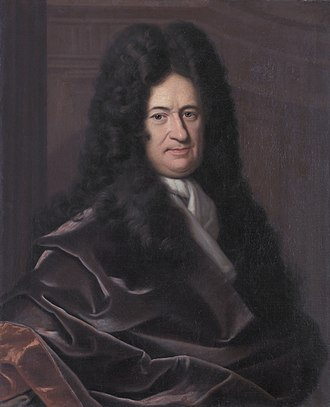
\includegraphics[width=0.45\textwidth]{figures/Gottfried_Wilhelm_Leibniz,_Bernhard_Christoph_Francke.jpg}
    \caption{Retrato de Gottfried Leibniz.\\Fuente: \href{https://es.wikipedia.org/wiki/Gottfried_Leibniz}{Wikipedia}}
    \label{fig:gottfried-leibniz}
\end{figure}

Aunque realmente la historia comienza en 1943 con la investigación de {Warren McCulloch} y {Walter Pitss}, publicaron el artículo \textit{A logical calculus of the ideas immanent in nervous activity} \cite{mcculloch1943logical}.
Dicho artículo creó distintas ramas de investigación (ordenadores digitales, inteligencia artificial, funcionamiento del perceptron).

\begin{figure}[H]
    \centering
    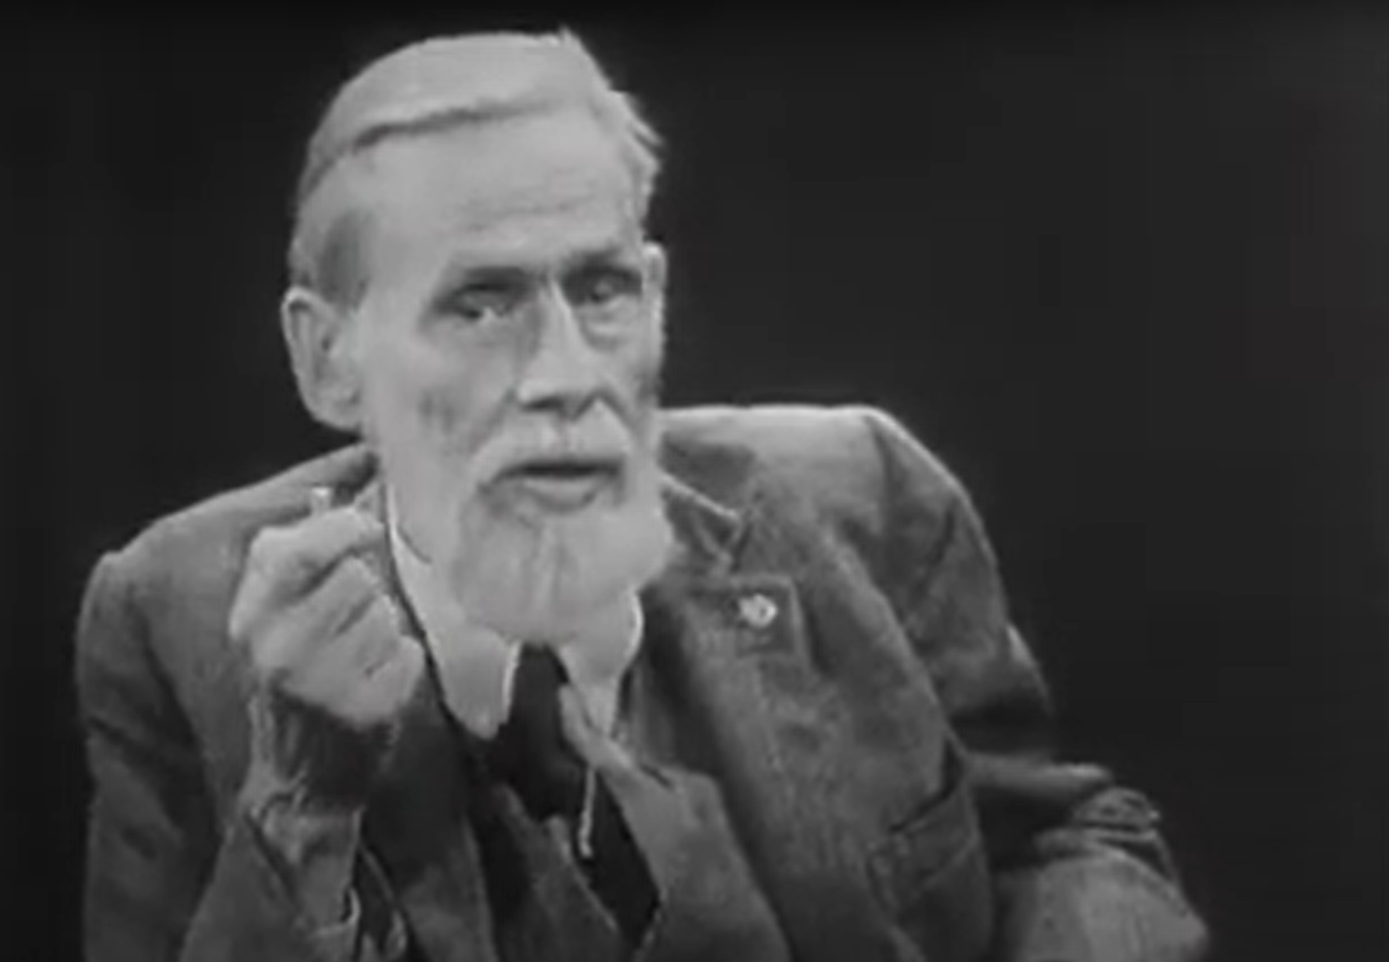
\includegraphics[width=0.65\textwidth]{figures/Warren Sturgis McCulloch Interview.png}
    \caption{Warren Sturgis McCulloch Interview.\\Fuente: \href{https://www.youtube.com/watch?v=8Wdz1Tj5084}{Entrevista en 1969}}
    \label{fig:Warren Sturgis McCulloch}
\end{figure}


En 1956 en la primera conferencia de inteligencia artificial organizada por la fundación {Rochester}, se reúnen los investigadores fundadores de los conceptos actuales de la IA ({Minsky, McCarthy, Rochester, Shanon}), gran parte de la bibliografía se refiere a este punto como el origen y contacto de las redes neuronales artificiales.
En dicha conferencia (\textit{Nathaural Rochester}) presento el modelo de una red neuronal que fue el resultado de la investigación desarrollada por el equipo de investigación de IBM.

\begin{figure}[H]
    \centering
    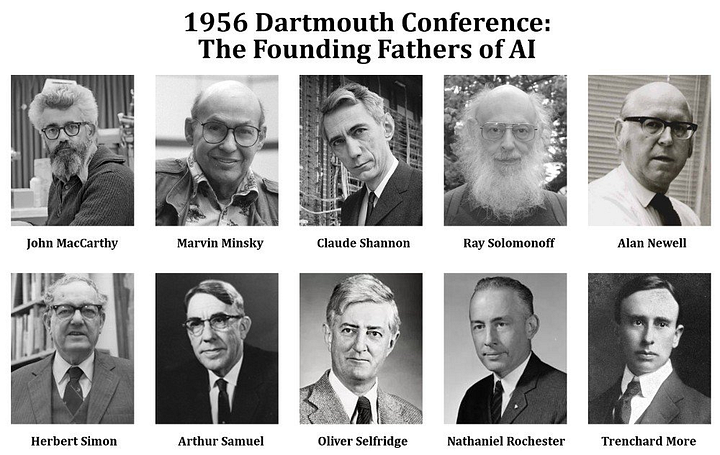
\includegraphics[width=0.75\textwidth]{figures/conferecia 1956 - 1689170718524.png}
    \caption{Los padres de la inteligencia artificial.\\Fuente: \href{https://www.linkedin.com/pulse/first-ever-ai-conference-tracing-evolution-history-ofai-nicky-verd}{Linkedin}}
    \label{fig:conferencia-1956}
\end{figure}

En 1957 se presenta el ``\textit{Perceptron}'' por {Frank Rosenblatt}, dicho elemento es un sistema clasificador de patrones, además contaba con la capacidad de aprender, de ser robusto matemáticamente y poder adaptarse si algún componente se dañaba.

\begin{figure}[H]
    \centering
    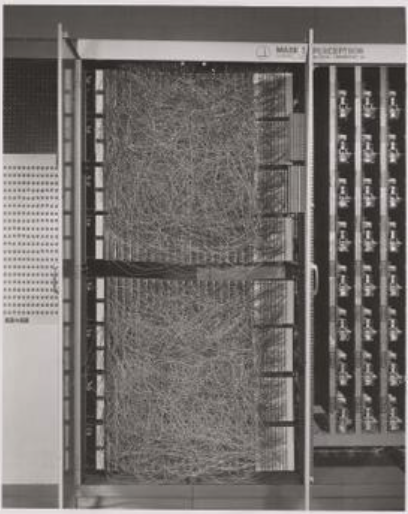
\includegraphics[width=0.4\textwidth]{figures/perceptron.png}
    \caption{Mark I Perceptron.\\Fuente: \href{https://en.wikipedia.org/wiki/Perceptron}{Wikipedia}}
    \label{fig:perceptron}
\end{figure}

El \textit{Perceptron} fue diseñado originalmente para el reconocimiento óptico usando un sistema de 400 fotocélulas en rejilla.
Posteriormente se describió el problema de no-linealidad que presentaban los perceptrones (Problema XOR) \cite{cuevastello2018apuntes}.

De 1959 a 1960 {Bernard Widrow} y {Ted Hoff} desarrollaron ``Adaline'' y ``Madaline'' \cite{widrow1960adaptive} que resolvía el problema de la no-linealidad y que tenía aplicación en el reconocimiento de voz, series temporales, caracteres, etc.

Posteriormente el \textit{MIT} realizo una investigación matemática muy crítica de todos los problemas que presentaba el \textit{Perceptron} llegando a la conclusión que tenían grandes problemas que no podrían ser resueltos, por lo que en la próxima década (años 60) se redujo drásticamente las investigaciones sobre el campo de las redes neuronales.
Esto llevo a uno de los famosos inviernos de la inteligencia artificial (1974 - 1980).

\begin{figure}[H]
    \centering
    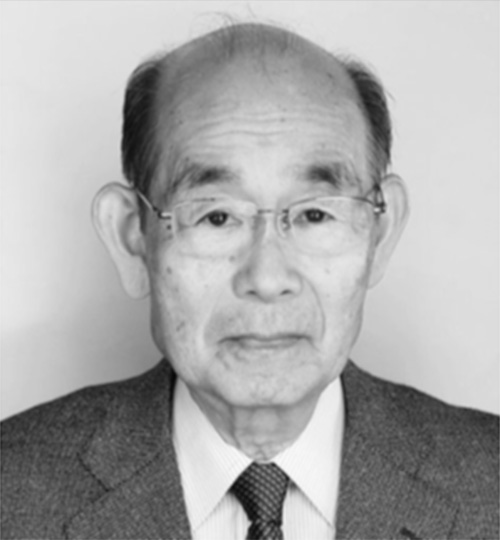
\includegraphics[width=0.25\textwidth]{figures/Kunihiko Fukushima.jpg}
    \caption{Kunihiko Fukushima.\\Fuente: \href{https://www.ieice.org/eng/about_ieice/new_honorary_members_award_winners/2017/meiyo_05e.html}{IEICE}}
    \label{fig:kunihiko-fukushima}
\end{figure}

Durante la década de los 70 se hacen aportes a la teoría \textit{Hebbiana}, se aportan logros en al análisis y descripción de reglas adaptativas, además de otros aportes al principio de aprendizaje competitivo.
En 1979 presentó {Kunihiko Fukushima} la primera red neuronal \gls{CNN}, la llamó Neocognitron \cite{fukushima1979neural}, dicho trabajo en un futuro se mejoraría con técnicas de \gls{BP-NN}.

En la década de los 80 se realizaron aportes como el algoritmo de \gls{BP-NN} que surgió del artículo de {Hopfield} \cite{hopfield1982neural}, esto despertó la curiosidad de muchos investigadores a volver al campo de las redes neuronales.
Se realizaron aportes como las redes \gls{GNN}.
La investigación continuó con {Stephen Grossberg} que realizo aportes derivados de estudios fisiológicos de cómo funcionaban las neuronas y la plasticidad, lo que permitió la creación de reglas y postulados, esto se ve en los trabajos de las redes \acrshort{art-nn} \cite{grossberg1987competitive}.
La investigación de {Hopfield} basada en el trabajo de {Stephen Grossberg} creo un sistema computacional neuronal interconectado que tiende a un mínimo de energía.
En 1985 {David E. Rumelhart} basándose en la investigación realizada por {Paul Werbos} \cite{etde_5080493} realizo un análisis experimental del algoritmo \gls{BP-NN} y su aplicación en redes \acrshort{fnn} \cite{rumelhart1985learning}.

{Yann LeCun} junto a su equipo, en 1989 crearon la primera aplicación \gls{CNN} con técnicas \gls{BP} dicha aplicación podía reconocer números a partir de imágenes.

\begin{figure}[H]
    \centering
    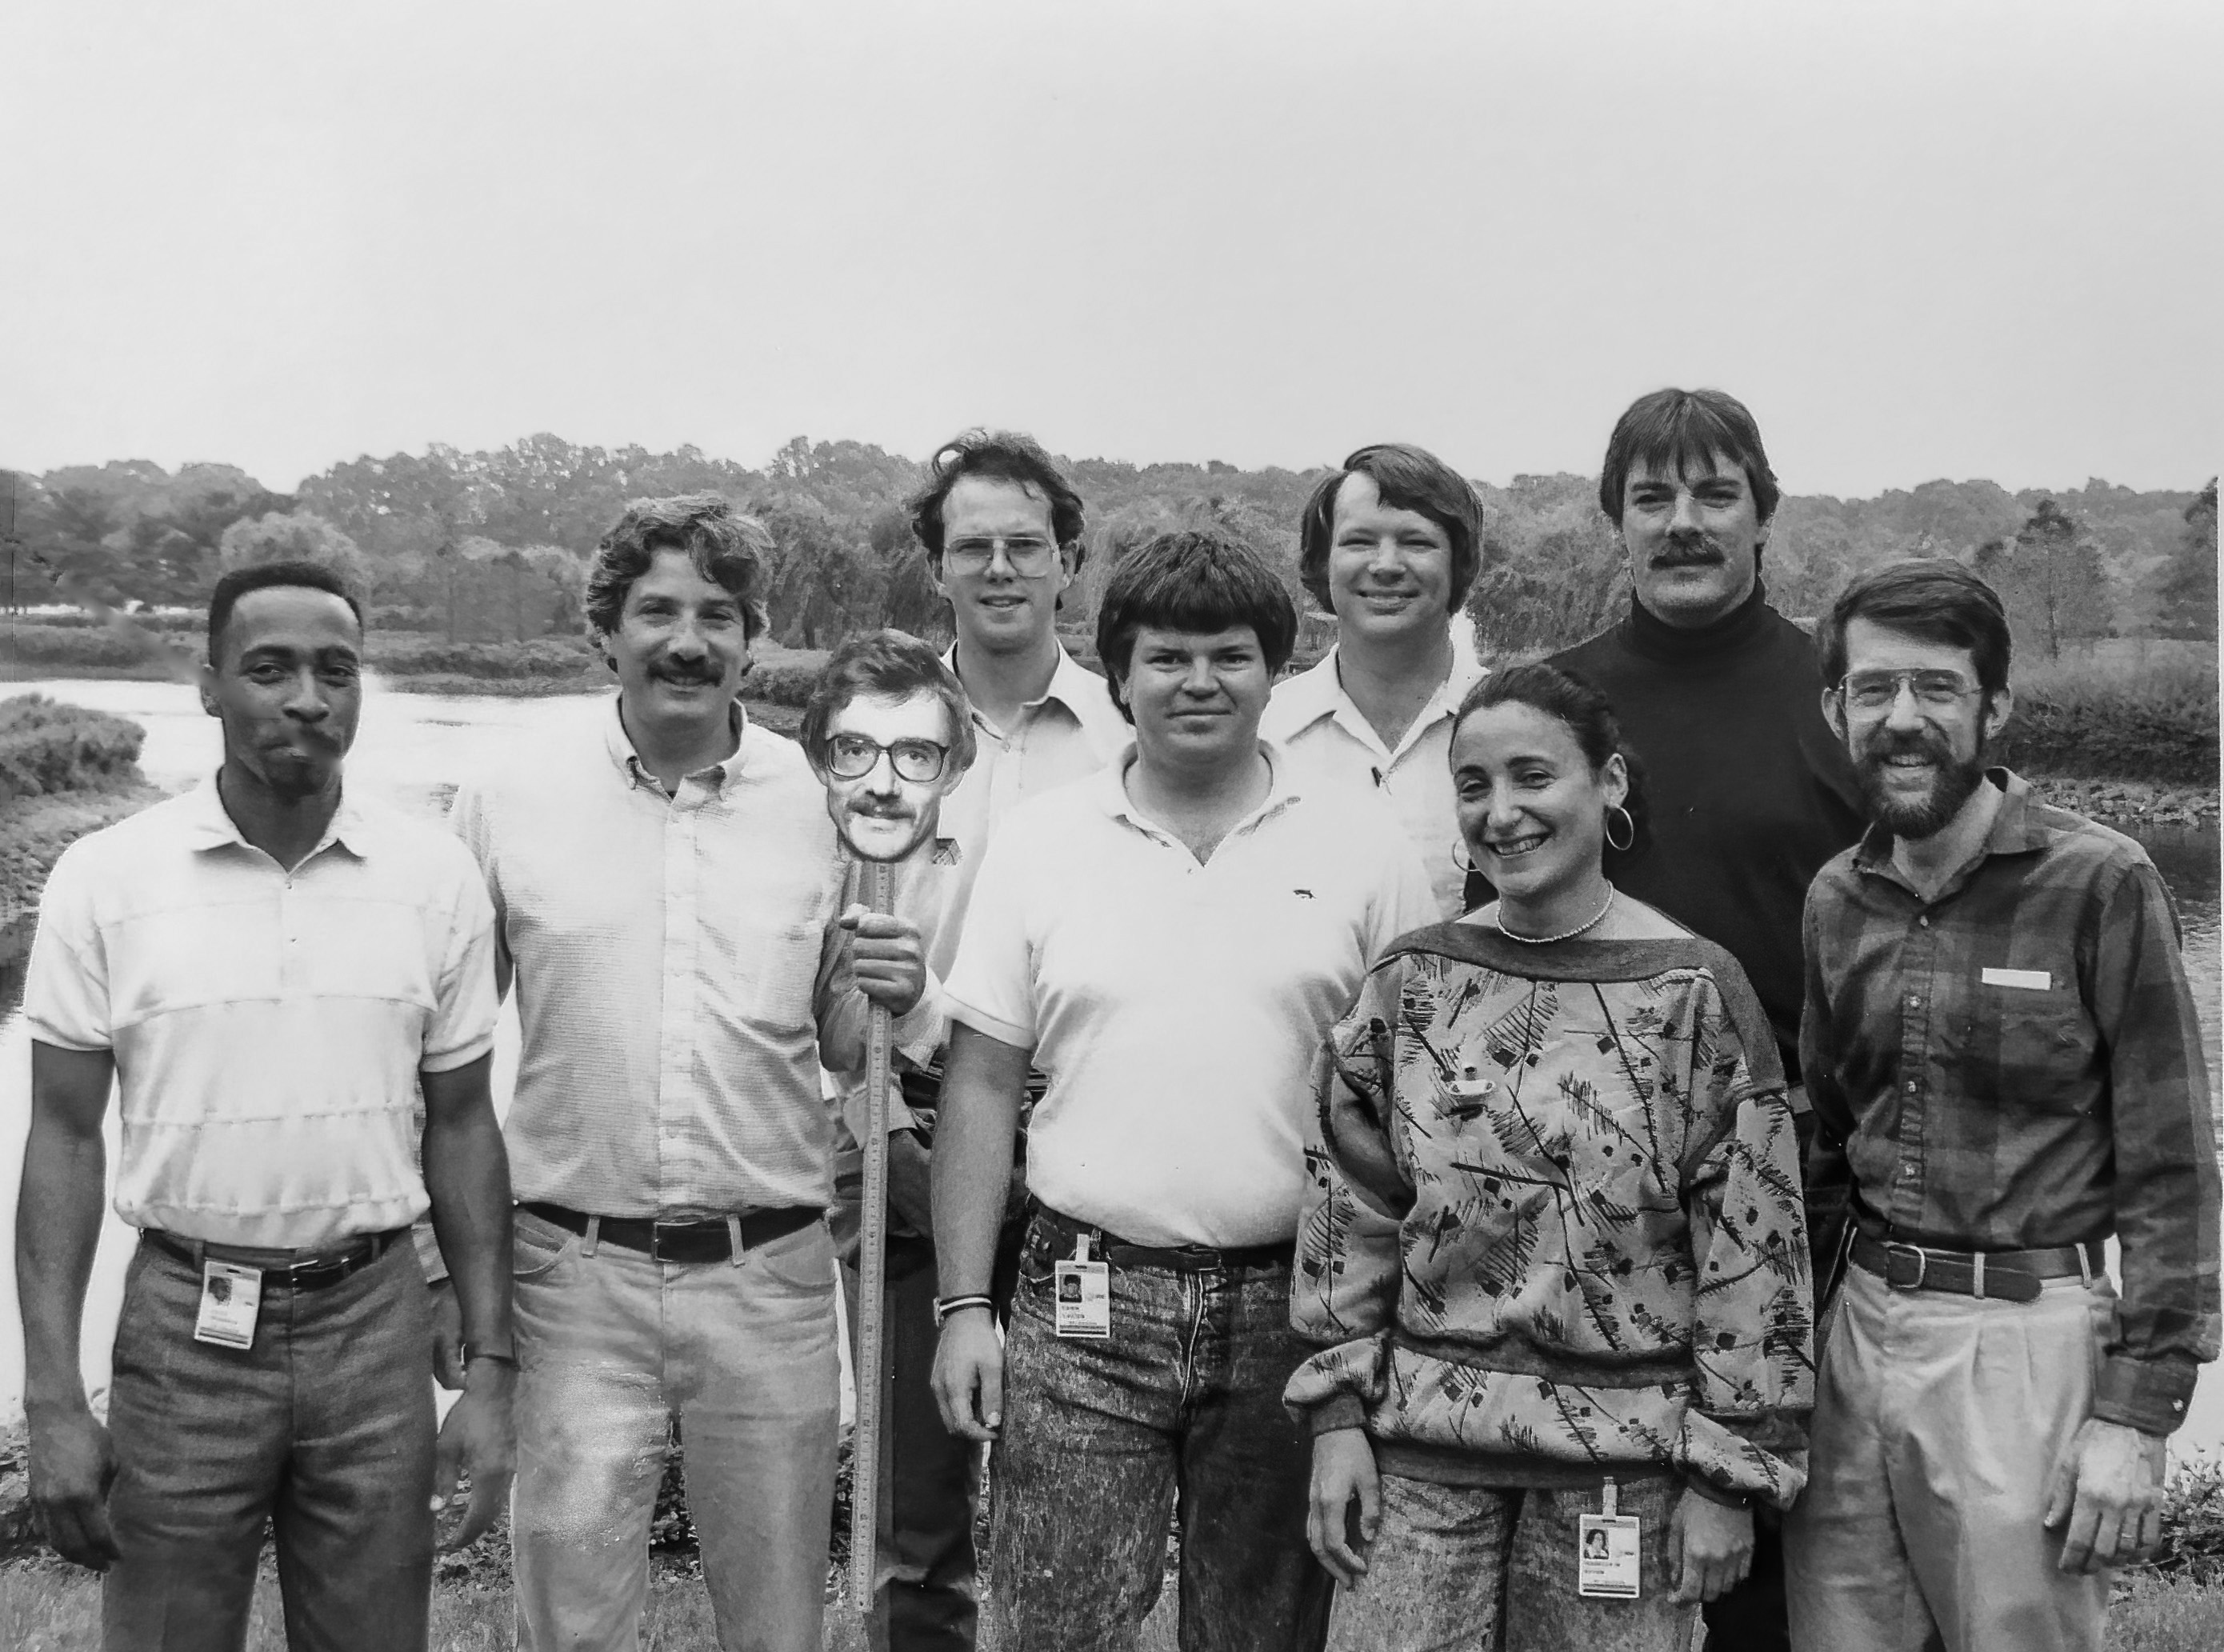
\includegraphics[width=0.65\textwidth]{figures/yann-lecun - EyIwmEDW8AIQs1C.jpeg}
    \caption{Adaptive Systems Research Department at Bell Labs 1989.\\Fuente: \href{https://twitter.com/ylecun/status/1378718317695934465}{Twitter Yann Lecun}}
    \label{fig:adaptive-systems-research-department-at-bell-labs}
\end{figure}

En la década de los 90 se presentaron múltiples investigaciones y muchos avances en el campo, uno de los más importantes fue la presentación de la primera \acrshort{gan} como una curiosidad, ya que se presentó como un duelo entre dos redes neuronales, en un principio fue un generador probabilístico y un predictor con el objetivo de maximizar la pérdida de cada uno en un juego \textit{minimax}.

En 1991 se presentó el trabajo \textit{Predictability Minimization} \cite{urgen1991learning} dichas técnicas sirvieron de inspiración para el aprendizaje por refuerzo,
En marzo de 1991 se hizo una aproximación a los \textit{transformers} con auto atención, lograron separar el conocimiento del control como una máquina clásica, pero de una forma completamente neuronal, además de gestionar actualizaciones de los pesos de forma muy rápida y eficiente.

Durante la década de 1990 las redes neuronales tendían a ser muy sencillas, con pocas capas y no muy complejas por las limitaciones técnicas de la época.
Por lo que muchos investigadores propusieron soluciones similares a las redes \acrshort{rnn} que permitían una retroalimentación, además de aceptar secuencias de información arbitraria.
Otros propusieron soluciones como la jerarquía de \acrshort{rnn} autosupervisada que aprende representaciones en distintos niveles de abstracción.
Comienzan a proponerse redes similares a las que en un futuro se llamarían \acrshort{dbn} como un método no supervisado para \acrshort{fnn}.

En junio de 1991 {Sepp Hochreiter} Figura \ref{fig:sepp-hochreiter} implemento el primer compresor de redes neuronales, además demostró uno de los principales problemas de las \acrshort{nn} el llamado problema del desvanecimiento o explosión del gradiente \ref{sec:gradient-descent} que hacía que el aprendizaje fallará.
Un análisis posterior condujo a los investigadores a una primera aproximación \acrshort{lstm}, aunque no sería hasta 1997 con la revisión por pares y publicación del artículo \textit{Long short-term memory} \cite{hochreiter1997long} que se solucionaría parcialmente el problema.

\begin{figure}[H]
    \centering
    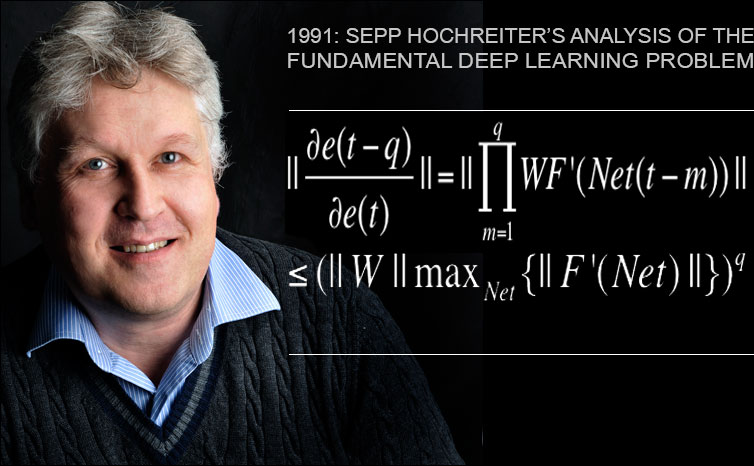
\includegraphics[width=0.65\textwidth]{figures/Sepp Hochreiter.jpg}
    \caption{Sepp Hochreiter.\\Fuente: \href{https://people.idsia.ch/~juergen/fundamentaldeeplearningproblem.html}{IDSIA}}
    \label{fig:sepp-hochreiter}
\end{figure}

Más adelante en el 2014 {Goodfellow} Figura \ref{fig:gan-ian-goodfellow} presento la primera red neuronal \acrshort{gan} pura para la generación de imágenes mediante el enfrentamiento de una red neuronal generativa contra una red neuronal discriminante entrenadas con el mismo conjunto de datos \cite{goodfellow2014generative}.
Durante los próximos años se realizaron muchos aportes a las redes neuronales generativas, principalmente de paralelización de los cálculos, técnicas de estabilización, generación condiciona, arquitecturas más eficientes, funciones de pérdidas más adecuadas, aplicaciones específicas (cambiar el estilo de pintura), redes apiladas, etc.
Fruto de todo ello {NVIDIA} en 2018 presento \gls{StyleGAN} \cite{karras2019stylebased} aunque publicaron el código en 2019 con fuertes mejoras.

\begin{figure}[H]
    \centering
    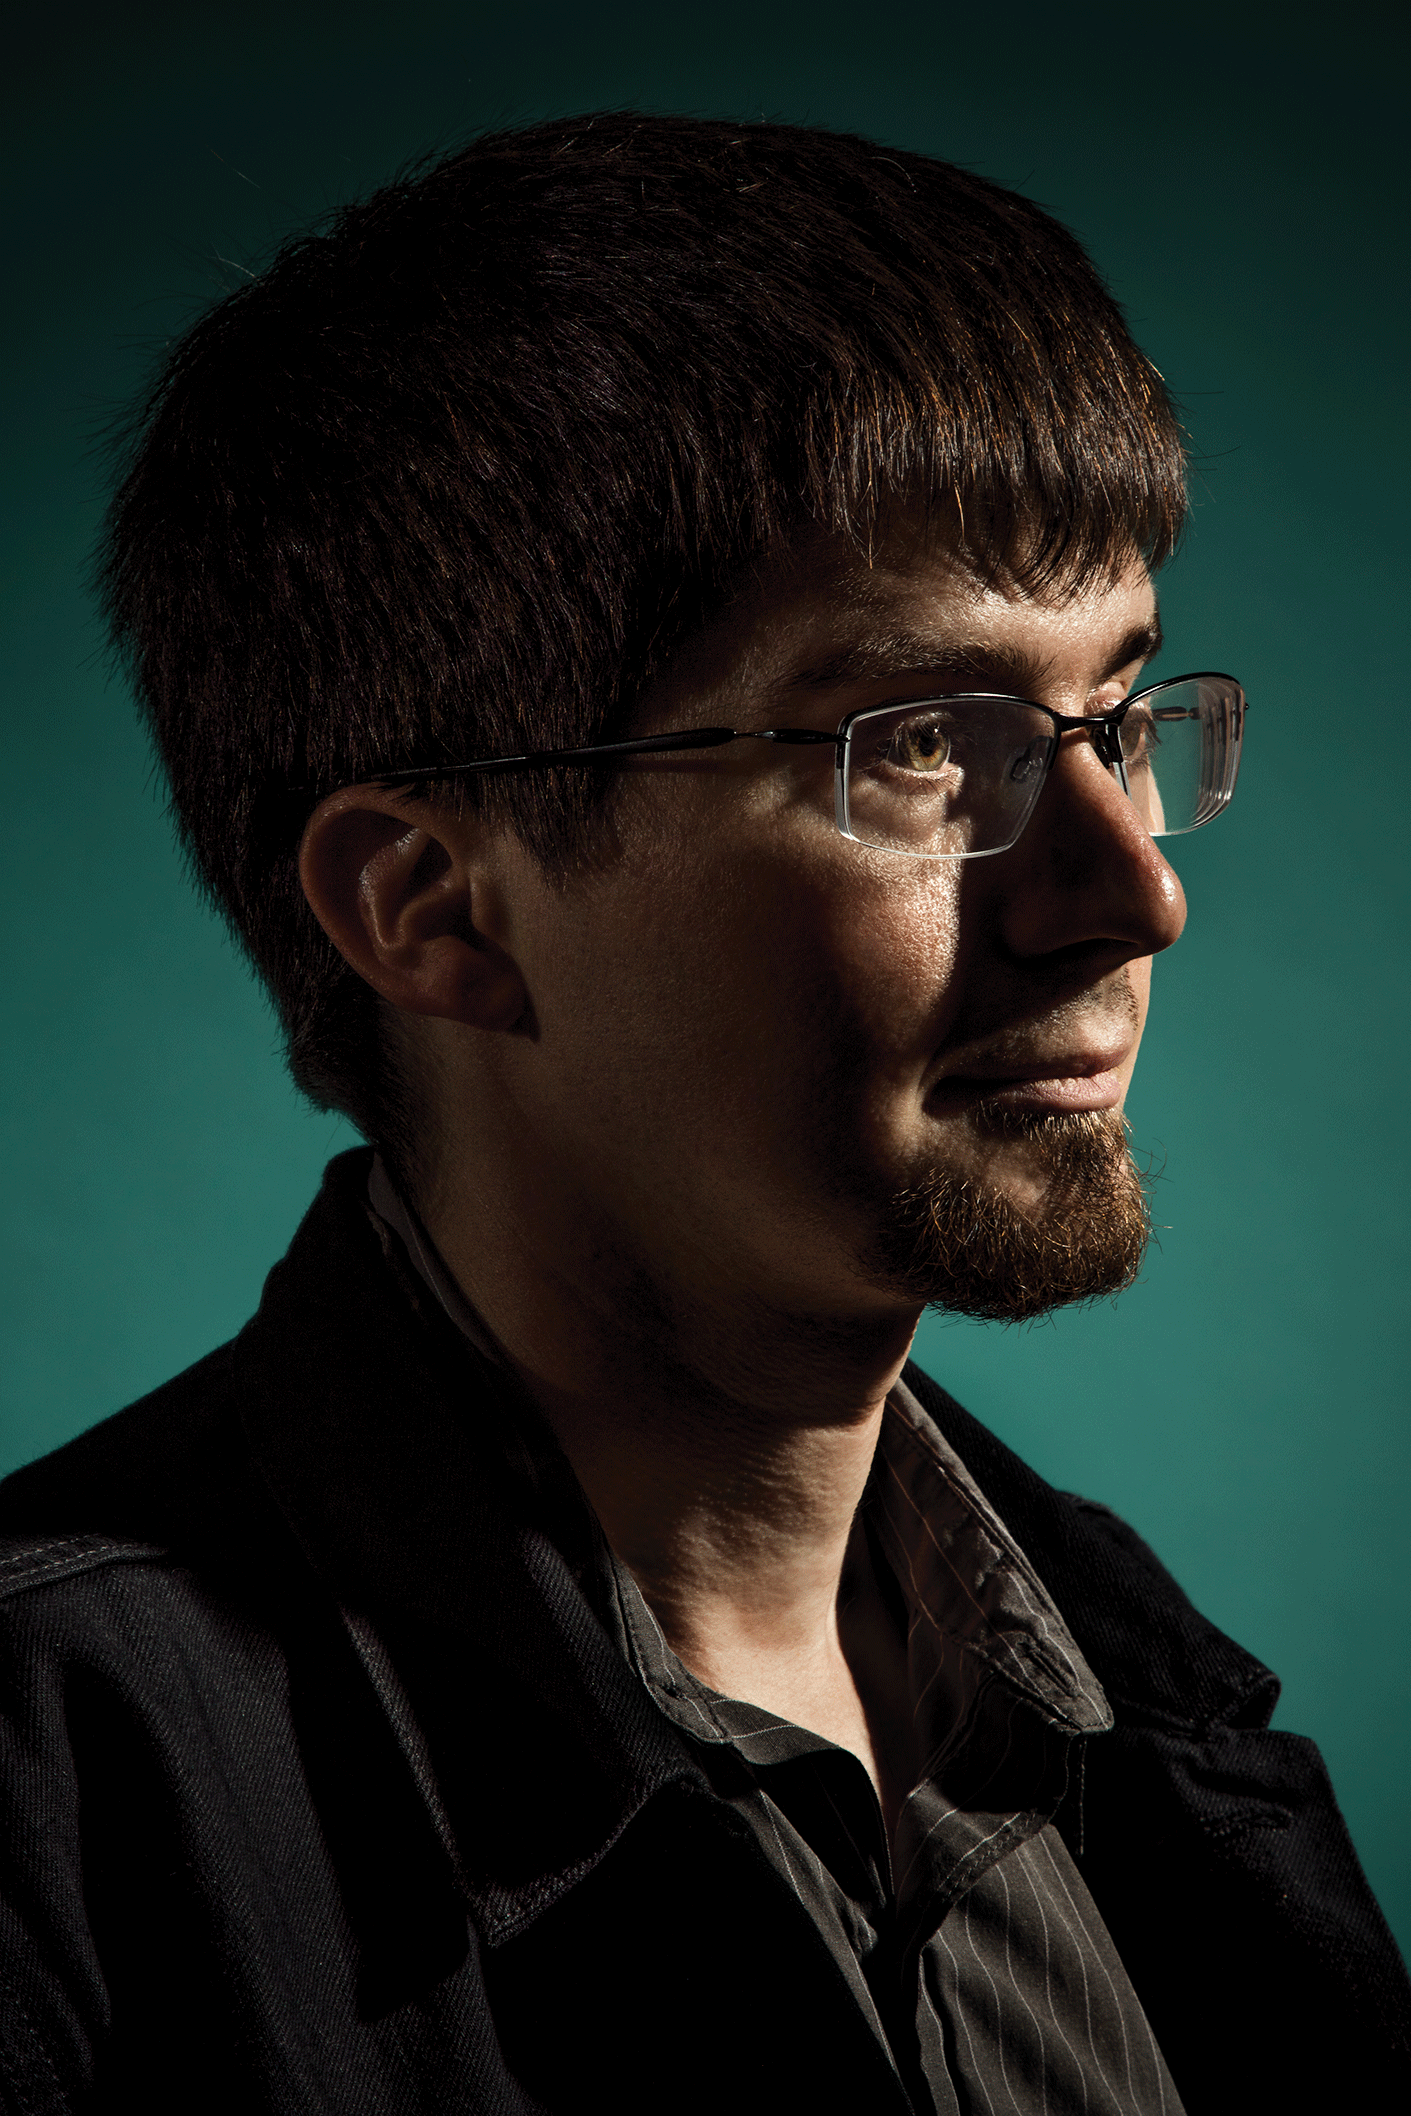
\includegraphics[width=0.2\textwidth]{figures/gan-goodfellow.png}
    \caption{Ian Goodfellow.\\Fuente: \href{https://www.technologyreview.es/s/10016/el-senor-de-las-gan-el-hombre-que-dio-imaginacion-las-maquinas}{MIT Technology Review}}
    \label{fig:gan-ian-goodfellow}
\end{figure}
% endregion


\section{Estado del arte}
\label{ch:2:section:state-of-the-art}

% region Teoría
\subsection{La ciencia de datos}
La ciencia de datos (\textit{Data Science}) es el estudio de los datos con el objetivo de extraer información útil, se usa principalmente para dar información útil a empresas. Es un campo multidisciplinar, ya que combina campos de las matemáticas, estadística e inteligencia artificial para analizar grandes cantidades de datos. Esto tiene como objetivo responder a las siguientes cuestiones: \textit{¿Qué paso?, ¿Por qué pasó?, ¿Qué pasará? O ¿Qué se puede hacer con los resultados?} \cite{aws-data-science}

La ciencia de datos analiza los datos de distintas formas.

\begin{enumerate}
    \item \textbf{Análisis descriptivo}: examina datos con visualizaciones (gráficos, tablas) para entender eventos pasados o actuales.
    \item \textbf{Análisis de diagnóstico}: profundiza en los datos para entender las razones detrás del evento. Emplea técnicas cómo descubrimiento de datos o correlaciones.
    \item \textbf{Análisis predictivo}: utiliza datos históricos y técnicas como machine learning para hacer predicciones precisas sobre patrones futuros.
    \item \textbf{Análisis prescriptivo}: busca la mejor respuesta para un resultado esperado. Utiliza técnicas como simulación y redes neuronales para recomendar el mejor curso de acción entre varias alternativas.
\end{enumerate}


\subsection{La minería de datos}
% Fases de la extracción del conocimiento 
% Dentro del KDD está la {minería de datos}

La minería de datos, es una técnica asistida por computadora, procesa grandes conjuntos de datos para descubrir patrones y relaciones ocultas. Este conocimiento resultante se aplica en la resolución de problemas, análisis de decisiones empresariales, etc. Esta técnica tiene distintas fases para procesar y extraer información útil.

\begin{enumerate}
    \item Comprender, identificar y definir el alcance del proyecto.
    \item Comprender los datos.
    \item Depurar datos (limpiar, integrar y dar formato).
    \item Modelar datos.
    \item Evaluar los resultados.
    \item Implementar resultados.
\end{enumerate}

La minería de datos es distinta en función de los datos y el objetivo, la mayoría del estado del arte segmenta la minería en tres tipos, minería de procesos, minería de textos y minería predictiva.

El Descubrimiento de Conocimientos en Bases de Datos \gls{KDD} es un proceso que utiliza algoritmos de minería de datos para explorar y extraer conocimientos útiles de grandes bases de datos. Con el avance tecnológico, se emplean técnicas de inteligencia artificial para este propósito, con el objetivo final de obtener conocimiento de alto nivel a partir de datos de bajo nivel. La Figura \ref{fig:kdd} esquematiza el proceso general del \textit{KDD}.

\begin{figure}[H]
    \centering
    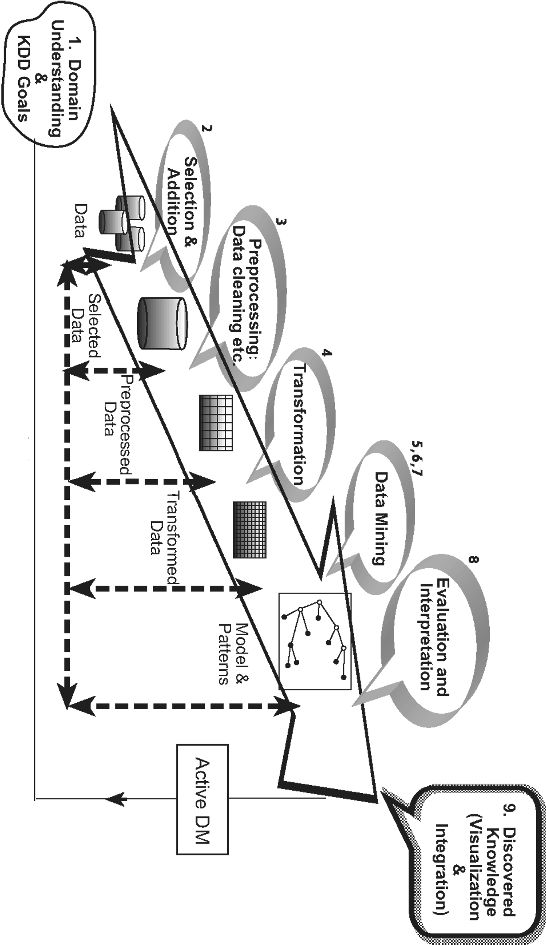
\includegraphics[angle=90,width=0.8\textwidth]{figures/chapter02/KDD.jpg}
    \caption{El proceso de descubrimiento de conocimiento en bases de datos.\\Fuente: Sección \textit{Introduction to Knowledge Discovery and Data Mining} \cite{rokach2010data}}
    \label{fig:kdd}
\end{figure}


\begin{enumerate}
    \item \textbf{Comprensión del Dominio de Aplicación}: se debe comprender los datos que se tratan y el campo de obtención con el objetivo de preparar los datos.
    \item \textbf{Selección y Creación de Conjunto de Datos}: se han de seleccionar los datos relevantes (Selección de características).
    \item \textbf{Preprocesamiento y Limpieza de Datos}: se han de eliminar las características no relevantes, datos perturbados, entradas incoherentes o tratar datos faltantes, etc. con el objetivo de obtener datos más limpios.
    \item \textbf{Transformación de Datos}: se deben tratar los datos, reduciendo la dimensionalidad, filtración, descomponiendo, etc. para que sea más sencillo el consumo de estos datos por una aplicación.
    \item \textbf{Elección de Tarea de Minería de Datos}: en función de los datos y del objetivo deberemos realizar una tarea (clasificación, regresión o agrupación), ya que en la minería de datos hay dos objetivos principales, \textbf{predicción} y \textbf{descripción}.
    \item \textbf{Elección del Algoritmo de Minería de Datos}: deberemos elegir entre los distintos algoritmos que se usan en la minería de datos, si buscamos precisión podemos usar redes neuronales, si buscamos explicabilidad podemos usar árboles de decisión.
    \item \textbf{Implementación del Algoritmo de Minería de Datos}: emplearemos el algoritmo seleccionado ajustando los parámetros para que nos del mejor resultado.
    \item \textbf{Evaluación de Patrones Minados}: debemos interpretar los resultados (reglas, confiabilidad, etc.) si no cumplen los objetivos que se buscaban en el primer paso deberemos reajustar toda la metodología, desde ajustar la selección de características a la interpretación o compresibilidad del modelo.
    \item \textbf{Utilización del Conocimiento Descubierto}: por último, debemos incorporar el conocimiento a los sistemas de toma de decisiones, este es el paso más importante, ya que con él podemos medir los efectos del conocimiento obtenido. Puede suceder que una vez implementado el modelo en sistema de producción pierda eficiencia si las condiciones reales son distintas a las de la creación del modelo.
\end{enumerate}


\begin{figure}[H]
    \centering
    \centerline{\includesvg[width=1\linewidth]{figures/chapter02/data-mining-taxonomy.drawio.svg}}
    \caption{Taxonomía de minería de datos.\\Fuente: Elaboración propia, inspirado en la sección \textit{Introduction to Knowledge Discovery and Data Mining} \cite{maimon2005data}}
    \label{fig:data-mining-taxonomy}
\end{figure}

La minería de datos puede estar orientada a la verificación o al descubrimiento de patrones, se debe automatizar su identificación, pudiendo usar un enfoque predictictivo o descriptivo. Para el descubrimiento se usa el aprendizaje inductivo, mientras que en la verificación se ha de evaluar las hipótesis externas usando métodos estadísticos clásicos. La terminología clásica del aprendizaje automático está clasificado en supervisado (clasificación y regresión) y no supervisado (agrupamiento), aunque existen muchos más términos en la terminología moderna esto podemos analizarlo más en profundidad en el libro \textit{Data Mining and Knowledge Discovery Handbook} \cite{maimon2005data}.


\subsection{Aprendizaje automático - \textit{Machine Learning}}

El \textit{machine learning} es la ciencia o rama de la inteligencia artificial que desarrolla, modelos estadísticos, desarrolla algoritmos que generalizan comportamientos y reconocen patrones. Es decir, hace posible el aprendizaje autónomo de las máquinas para realizar tareas sin la necesidad programar las instrucciones explícitamente. El \textit{machine learning} busca procesar grandes cantidades de datos e identificar patrones de datos de forma automática.

\begin{figure}[H]
    \centering
    \centerline{\includesvg[width=0.75\linewidth]{figures/chapter02/machine-learning-rules.drawio.svg}}
    \caption{El \textit{Machine Learning} como paradigma de programación.\newline{}Fuente: Elaboración propia.}
    \label{fig:machine-learning-rules}
\end{figure}

Como podemos ver en la Figura \ref{fig:machine-learning-rules} en el paradigma clásico se necesitaba conocer el dominio de los datos y las reglas en profundidad y programar los descriptores de forma manual para procesar los datos. En el paradigma del \textit{machine learning} permite extraer esas reglas y patrones para procesar nuevos datos a partir de respuestas que conocíamos previamente, estas respuestas previas deben ser extraídas o validadas por expertos.

Una clasificación de las tareas del \textit{machine learning} lo podemos ver en la Figura \ref{fig:machine-learning}, esta clasificación está dividida en función de cómo se realiza el aprendizaje del modelo.

\begin{figure}[H]
    \centering
    \centerline{\includesvg[width=1\linewidth]{figures/chapter02/machine-learning.drawio.svg}}
    \caption{Clasificación de los algoritmos de aprendizaje automático.\\Fuente: Elaboración propia.}
    \label{fig:machine-learning}
\end{figure}

El \textit{machine learning} puede trabajar con datos estructurados y no estructurados, aunque estos últimos requieren un procesamiento previo para adaptarlos en un formato estructurado.



\subsection{Aprendizaje profundo - \textit{Deep Learning}}
% TODO: Explicar el Deep Learning https://idus.us.es/bitstream/handle/11441/90004/Centeno%20Franco%20Alba%20TFG.pdf

El \textit{deep learning} es una subrama del \textit{machine learning} que usa redes neuronales artificiales para analizar datos no lineales, estas redes imitan el comportamiento del cerebro humano, para esto suelen contar con arquitecturas complejas.
Se distingue del \textit{machine learning} por los tipos de datos con los que puede trabajar y por los métodos con los que hace que los modelos aprendan.

Otra de las características que diferencia al \textit{deep learning} del \textit{machine learning} es que elimina parte del procesamiento previo de datos, ya que sus algoritmos pueden ingerir y procesar datos no estructurados.


%  ============================================================================================================================================================
%  ============================================================================================================================================================
%  ============================================================================================================================================================

% https://learning.oreilly.com/library/view/neural-networks-and/9781492037354/ch01.html#idm139624964652336
\subsection{Redes neuronales artificiales - \textit{Artificial Neuronal Networks}}
% TODO: \cite{ibm-deep-learning}
% Explicar uso de múltiples neuronas artificiales para crear capas y luego redes
El \textit{deep learning} emplea principalmente redes neuronales para reconocer, clasificar y describir con precisión patrones de datos. Estas redes están inspiradas en el funcionamiento del cerebro humano.  \cite{ibm-deep-learning}

Las redes neuronales es un conjunto de neuronas artificiales que están organizadas generalmente por capas. Estas redes tienen una capa de entrada, una capa de salida y múltiples capas ocultas con distintas funciones de activación que ponderan los pesos de cada neurona.

Existen formas muy variadas de componer las capas, a esto se le denomina \textbf{topología de red neuronal}, en función del objetivo que se busque, la topología será muy distinta.

\subsubsection{Elementos de una neurona artificial}

Como se ha comentado previamente las neuronas artificiales están inspiradas en las neuronas biológicas del cerebro humano, fueron los investigadores \textit{McCulloch} y \textit{Pitts} \cite{mcculloch1943logical} los que sentaron las bases de lo que es una neurona artificial, demostrando que su modelo de red neuronal podía realizar cálculos que se correspondían con la lógica proposicional.

% TODO explicar las partes que propusieron \textit{McCulloch} y \textit{Pitts} 

\begin{figure}[H]
    \centering
    \centerline{\includesvg[width=1\linewidth]{figures/chapter02/artificial-neuron.drawio.svg}}
    \caption{Partes de una neurona artificial bioinspirada en una neurona biológica.\\Fuente: Elaboración propia}
    \label{fig:artificial-neuron}
\end{figure}

En la Figura \ref{fig:artificial-neuron} podemos ver las distintas partes de una única neurona artificial y sus partes equivalentes con una neurona biológica. El axón opera como la entrada de información a la neurona, la sinapsis como las conexiones con la neurona que son los pesos, el cuerpo celular como la neurona que representa la unidad de procesamiento central donde se pondera la suma de las señales de entrada, el cuello del axón sería nuestra función de activación que se activa cuando supera un umbral y el axón sería nuestra señal de salida.



% perceptron simple
% perceptron multicapa
% Funciones de optimización
% Funciones de activación
% Funciones de perdida
% Capas
% Tipologías
% Descenso de gradiente



\subsubsection{Funcionamiento de una red neuronal\label{neural-network}}

Las redes neuronales profundas tienen multitud de capas con nodos interconectados, cada capa sobre la capa anterior con el objetivo de optimizar la precisión de una perdición o clasificación. A esta progresión de cálculos se le denomina ``propagación hacia delante''.

El proceso de ``propagación inversa'' es el encargado de calcular errores de precisión, ajustar sesgos y ponderaciones usando algoritmos como \nameref{sec:gradient-descent}.

La capa de entrada es por donde el modelo ingiere los datos, y la capa de salida es donde el modelo responderá con la predicción o clasificación una vez se haya completado la fase de aprendizaje.

\begin{figure}[H]
    \centering
    \centerline{\includesvg[width=1\linewidth]{figures/chapter02/neuronal-network.drawio.svg}}
    \caption{Red neuronal artificial.\\Fuente: Elaboración propia}
    \label{fig:artificial-neuronal-network}
\end{figure}

En la Figura \ref{fig:artificial-neuronal-network} podemos ver una arquitectura simple de una red neuronal que cuenta con la capa de entrada, la capa de salida y dos capas ocultas.

El vector de entrada $X = (x_{1}, x_{2}, ..., x_{n})$ será la información suministrada a nuestra red a través de la capa de entrada, este vector será de tamaño $n$.

\begin{figure}[H]
    \centering
    \captionsetup{justification=centering}
    \centerline{\includesvg[width=1\linewidth]{figures/equations/Notation.drawio.svg}}
    \caption{Cálculo de los pesos de la red neuronal artificial.\\Fuente: Elaboración propia}
    \label{fig:notation}
\end{figure}

\begin{enumerate}
    \item Función de la red neuronal: $f(x) = W x + b$
    \item Matriz de pesos: $W = \left[w_{0,n}, w_{1,n}, ...,w_{m,n}\right]$
    \item Vector de pesos: $w_{n} \in \mathbb{R}^{D}$
    \item Vector de entrada: $x \in \mathbb{R}^{D}$
    \item Vector del bias: $b \in \mathbb{R}^{C}$
\end{enumerate}

% El proceso de reducción de dimensionalidad se lleva a cabo, para convertir el vector de características del espacio original en un nuevo espacio con un conjunto más pequeño, linealmente no correlacionadas mediante la siguiente función $f: \mathbb{R}^{D} \rightarrow \mathbb{R}^{C}$ con $C \ll D$, donde la red neuronal está expresada como $f(x) = W x + b$. Está red cuenta con las siguientes partes $\mathbf{W} = \left[w_{0}^{T}, w_{1}^{T}, ..., w_{C}^{T}\right]$ es la matriz de vectores de peso, que viene dada la expresión $\mathbf{w_{j}} \in \mathbb{R}^{D}$. El vector de entrada es $\mathbf{x} \in \mathbb{R}^{D}$ y el $bias$ es un vector que está definido en el espacio $\mathbf{b} \in \mathbb{R}^{C}$

\paragraph*{El perceptron simple}
% Definición
% Usos 
% algoritmo de entranmiento
% Problema XOR

El Perceptron es una neurna artificial simple llamada también como \gls{LTU}. La \gls{LTU} calcula una suma ponderada de los valores de las entradas $Z = w_{1} x_{1} + w_{2} x_{2} + \cdots + w_{n} x_{n}$ se aplica el umbral para generar el resultado.

La función umbral comun en \gls{LTU} es la función heaviside \ref{eq:heaviside}.

\noindent\begin{minipage}{0.45\textwidth}
    \begin{equation*}
        heaviside(z) =
        \begin{cases}
            0 & \textup{si } z < 0       \\
            1 & \textup{si } z \geq{}  0
        \end{cases}
    \end{equation*}
\end{minipage}
\begin{minipage}{0.45\textwidth}
    \begin{equation}
        sgn(z) =
        \begin{cases}
            -1 & \textup{si } z < 0  \\
            0  & \textup{si } z = 0  \\
            +1 & \textup{si } z >  0
        \end{cases}
        \label{eq:heaviside}
    \end{equation}
\end{minipage}

Se puede emplear para una clasificación binaria lineal simple, mediante una combinación lineal de las entradas; si la operación supera el umbral, se obtendrá un resultado binario en un vector.

El algoritmo de entrenamiento del Perceptrón se basa en ajustar los pesos de conexión entre las entradas y la neurona de salida para mejorar la precisión de las predicciones. Está inspirado en la regla de Hebb, que sugiere que las conexiones entre neuronas se fortalecen cuando una neurona activa repetidamente a otra.

Primero inicializa los pesos, predice, evalua su error y actualización de los pesos para en la siguiente iteración minimizar su error.

Rosenblatt demostro que el algoritmo convergeria hacia una solución, esto es llamado el Teorema de convergencia del perceptrón \cite{geron2018neural}.

Marvin Minsky y Seymour encontraron una serie de debilidades que los perceptrones son incapaces de resolver, algunas de estas debilidades se pueden resolver apilando varios perceptrones, la \gls{ANN} resultante se le llama \gls{MLP}.

Uno de los problemas clasicos que tenian los perceptrones simples era el problema de clasificación XOR, esto está representado en la Figura \ref{fig:problem-xor}. Como tal el perceptrón es un modelo que puede aprender funciones lineales, pero el problema XOR no es linealmente separable, lo que significa que no se puede trazar una línea recta para separar las dos clases (A y B) en el espacio de entrada binario de dos dimensiones.

\begin{figure}[H]
    \centering
    \centerline{\includesvg[width=0.35\linewidth]{figures/chapter02/tfm-xor-problem.drawio.svg}}
    \caption{Problema de clasificación XOR.\\Fuente: Elaboración propia}
    \label{fig:problem-xor}
\end{figure}


\paragraph*{El perceptron multicapa y retropropagación}

Fue en 1986 cuando {D. E. Rumelhart} propuso la retropropagación junto a multiples capas para resolver el problema de clasificación XOR.

El proceso es el siguiente, por cada instancia de entrenamiento se calcula la salida de cada neurona en la capa consecutiva (paso hacia adelante). A continuación se mide el error de salida de la red (la diferencia entre la salida deseada y la de la red) calculará cuánto contribuyo cada neurona en la última capa oculta al error de cada neurona de salida. Se mide cuantas contribuciones de error provienen de cada neurona en la capa oculta anterior, así sucesivamente hasta que se llega a la capa de entrada(paso hacia atras). Se mide eficientemente el gradiente de error en todos los pesos de la conexión en la red propagando el gradiente de error hacia atras. \cite{geron2018neural}

Este proceso funciona, ya que se cambió la función escalonada de las \gls{LTU} a una función logística Sigmoid \ref{eq:sigmoid}, esto se requeria, ya que la función de paso contiene solo segmentos planos y por tanto no habia gradientes. Esto permitio que el descenso de gradiente pudiera ir progresando lentamente hasta converger. El algoritmo de retroalimentación se puede usar con otras funciones de activación que veremos más adelante.


\subsubsection{El descenso de gradiente\label{sec:gradient-descent}}
% region El descenso de gradiente
% TODO: definición
% TODO: explicar el descenso de gradiente
% TODO: problema
El método de descenso de gradiente trata de encontrar un minimo en una función dada, ya sea local o global. El método usa el gradiente negativo ${-\nabla{f}}$, con este método obtenemos la dirección con el descenso máximo en los valores de la función, con esto buscamos encontrar la posición minima.

El problema de desvanecimiento y explosión de gradiente

\begin{figure}[H]
    \centering
    \centerline{\includesvg[width=0.6\linewidth]{figures/chapter02/fx_optimizer.svg}}
    \caption{Descenso de graidente\\Fuente: \href{https://fxdatalabs.com}{F(x) Data Labs Pvt. Ltd.}}
    \label{fig:gradient-descent}
\end{figure}

% endregion El descenso de gradiente


\subsubsection{Optimizadores\label{optimizers}}
% region Optimizadores
% TODO: definición
% TODO: Tipos
% TODO: Usos
Los optimizadores son los algoritmos que buscan encontrar la mejor solución para un problema esto se utilizan en conjunto con el descenso de gradiente para mejorar su eficiencia y rendimiento, generalmente minimizando o maximizando una función objetiva al ajustar sus parámetros. Existen muchos optimizadores que nos permiten explorar de forma eficiente el espacio de posibles soluciones.

% https://interactivechaos.com/es/manual/tutorial-de-machine-learning/adagrad

Estos son algunos de los optimizadores más famosos.
\begin{enumerate}
    \item \textbf{SGD} (Stochastic Gradient Descent with Momentum): Descenso de gradiente estocástico con momentum.
    \item \textbf{Adam} (Adaptive Moment Estimation): Descenso de gradiente con tasa de aprendizaje adaptativa.
    \item \textbf{Adamax} (Adaptive Moment Estimation with Infinity Norm):  variante de Adam que utiliza la norma infinita en lugar de la norma 2 para calcular y actualizar el término de escala máximo.
    \item \textbf{AdaGrad} (Adaptative Gradient Algorithm): variante de \textit{SGD} en la que se emplean distintas tasas de aprendizaje teniendo en cuenta el gradiente acumulado en cada una de las variables.
    \item \textbf{RMSprop} (Root Mean Square Propagation): variante de \textit{AdaGrad} en la que, en lugar de mantener un acumulado los gradientes, se utiliza el concepto de ``ventana'' para considerar los gradientes más recientes.
\end{enumerate}

% endregion Optimizadore

\subsubsection{Funciones de activación\label{sec:activations-functions}}
% region Funciones de activación
% TODO: definición, explicación y usos
% TODO: tipos, solo mostramos las más importantes
% TODO: 
Las funciones de activación son una función matemática que determina la salida de una neurona o nodo en función de su entrada, esto introduce no linealidad en el modelo y permitiendo que la red aprenda patrones complejos y mejora su capacidad de representación.

Existen muchas funciones de activación que modifican los pesos de la red neuronal de distintas formas.

\paragraph*{F. Activaciones no lineales - \textit{Non-linear Activations (weighted sum, nonlinearity)} \cite{pytorch2024github}}

\begin{enumerate}
    \item \textbf{ReLU}:
    \item[] \begin{equation} \varphi(x) = \operatorname*{max}(0,x) \end{equation}
    \item \textbf{LeakyReLU}:
    \item[] \begin{equation} \varphi(x) = \operatorname*{max}\left(0,x\right) + \operatorname*{negative\_slope} * \operatorname*{min}\left(0,x\right)  \end{equation}

    \item \textbf{Softplus}:
    \item[] \begin{equation} \varphi(x) = \frac{1}{\beta} \operatorname*{log}\left(1+e^{\beta x}\right) \end{equation}
    \item \textbf{SoftSign}:
    \item[] \begin{equation} \varphi(x) = \frac{x}{1+\lvert x \rvert} \end{equation}

    \item \textbf{Tanh}:
    \item[] \begin{equation} \varphi(x) = \frac{e^{x}-e^{-x}}{e^{x}+e^{-x}} \end{equation}
    \item \textbf{Sigmoid}:
    \item[] \begin{equation} \varphi(x) = \frac{1}{1+e^{-x}} \label{eq:sigmoid} \end{equation}
\end{enumerate}

\begin{figure}[H]
    \centering
    \captionsetup{justification=centering}

    \begin{subfigure}{.475\linewidth}
        \centering
        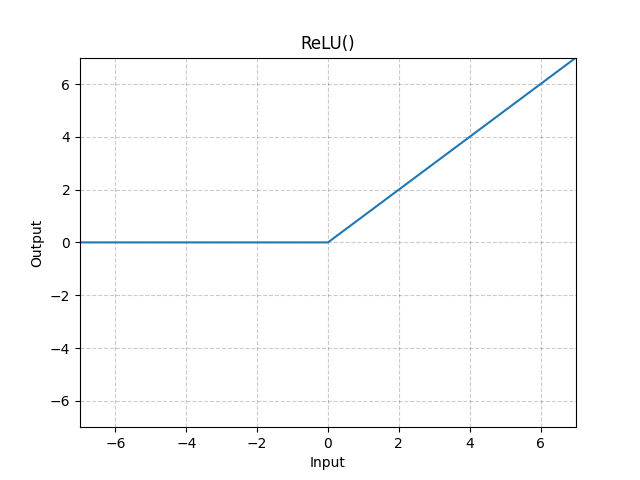
\includegraphics[width=0.75\linewidth]{figures/equations/ReLU.png}
        \caption{Función de activación ReLU.\newline{}Fuente: \href{https://pytorch.org/docs/stable/generated/torch.nn.ReLU.html}{Pytorch torch.nn.ReLU}}
        \label{subfig:torch.nn.ReLU}
    \end{subfigure}\hfill % <-- "\hfill"
    \begin{subfigure}{.475\linewidth}
        \centering
        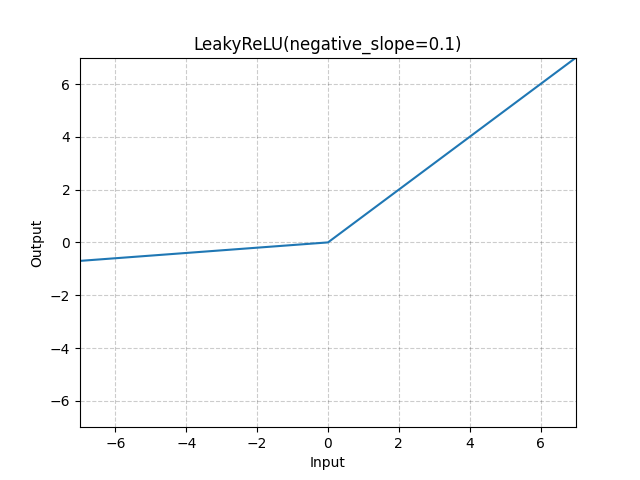
\includegraphics[width=0.75\linewidth]{figures/equations/LeakyReLU.png}
        \caption{Función de activación LeakyReLU.\newline{}Fuente: \href{https://pytorch.org/docs/stable/generated/torch.nn.LeakyReLU.html}{Pytorch torch.nn.LeakyReLU}}
        \label{subfig:torch.nn.LeakyReLU}
    \end{subfigure}

    \medskip % create some *vertical* separation between the graphs
    \begin{subfigure}{.475\linewidth}
        \centering
        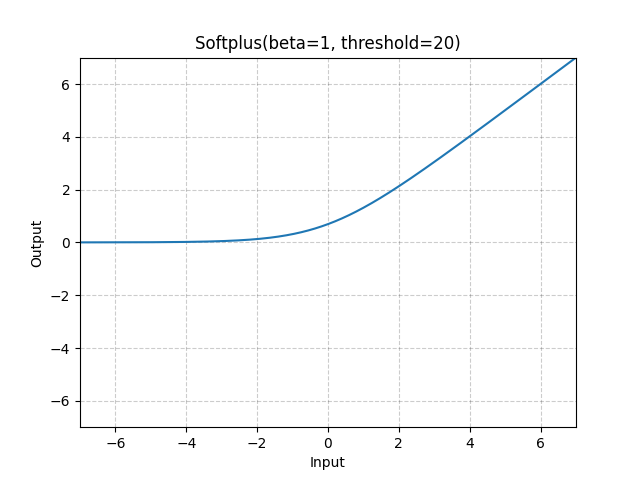
\includegraphics[width=0.75\linewidth]{figures/equations/Softplus.png}
        \caption{Función de activación Softplus.\newline{}Fuente: \href{https://pytorch.org/docs/stable/generated/torch.nn.Softplus.html}{Pytorch torch.nn.Softplus}}
        \label{subfig:torch.nn.Softplus}
    \end{subfigure}\hfill % <-- "\hfill"
    \begin{subfigure}{.475\linewidth}
        \centering
        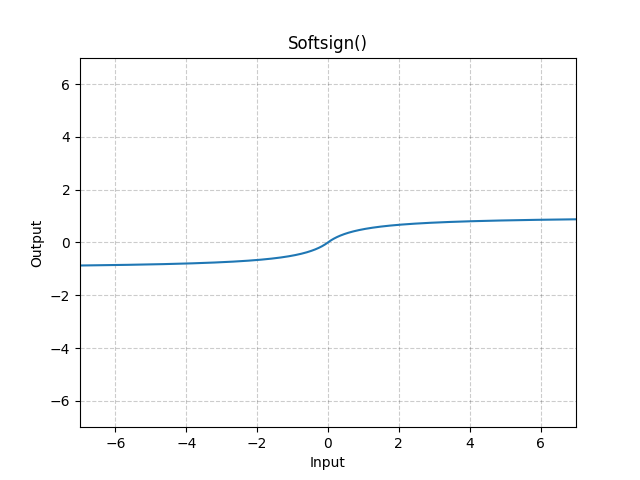
\includegraphics[width=0.75\linewidth]{figures/equations/Softsign.png}
        \caption{Función de activación Softsign.\newline{}Fuente: \href{https://pytorch.org/docs/stable/generated/torch.nn.Softsign.html}{Pytorch torch.nn.Softsign}}
        \label{subfig:torch.nn.Softsign}
    \end{subfigure}

    \medskip % create some *vertical* separation between the graphs
    \begin{subfigure}{.475\linewidth}
        \centering
        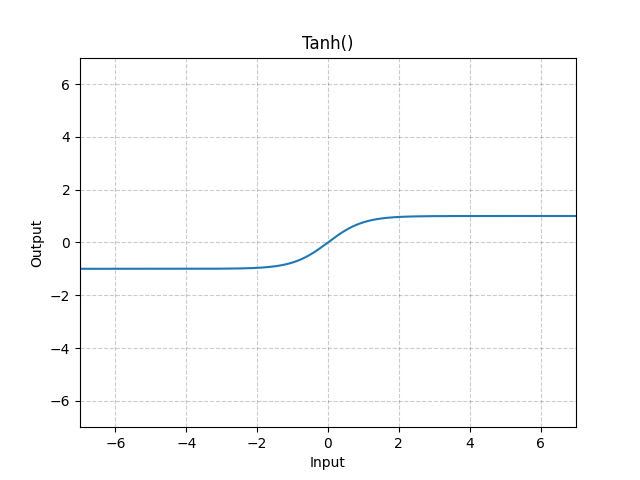
\includegraphics[width=0.75\linewidth]{figures/equations/Tanh.png}
        \caption{Función de activación Tanh.\newline{}Fuente: \href{https://pytorch.org/docs/stable/generated/torch.nn.Tanh.html}{Pytorch torch.nn.Tanh}}
        \label{subfig:torch.nn.Tanh}
    \end{subfigure}\hfill % <-- "\hfill"
    \begin{subfigure}{.475\linewidth}
        \centering
        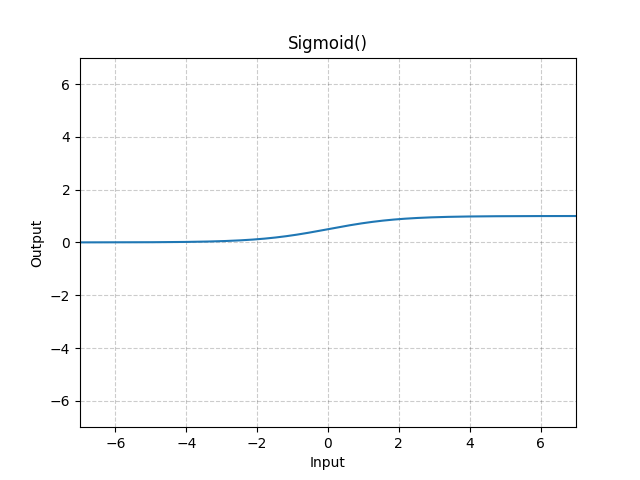
\includegraphics[width=0.75\linewidth]{figures/equations/Sigmoid.png}
        \caption{Función de activación Sigmoid.\newline{}Fuente: \href{https://pytorch.org/docs/stable/generated/torch.nn.Sigmoid.html}{Pytorch torch.nn.Sigmoid}}
        \label{subfig:torch.nn.Sigmoid}
    \end{subfigure}

    \caption{Funciones de activación no lineales}
    \label{fig:equations--Non-linear-Activations}
\end{figure}


\paragraph*{F. Activaciones no lineales - \textit{Non-linear Activations (other)} \cite{pytorch2024github}}
% TODO: explicar las funciones de activación no lineales más importantes

\begin{enumerate}
    \item \textbf{Softmax}: Aplica la función Softmax a un Tensor de entrada $n$-dimensional re-escalándolos para que los elementos del Tensor de salida $n$-dimensional se encuentren en el rango [0,1]. \cite{pytorch2024github}
    \item[] \begin{equation} \varphi(x_{i}) = \frac{e^{x_{i}}}{\sum_{j}{e_{j}}} \end{equation}
\end{enumerate}


% endregion Funciones de activación

\subsubsection{Tipos de capas}
% region Tipos de capas
% TODO: Capas de entrada, ocultas y de salida.
% TODO: Capas densas, no lineales con y sin pesos
% TODO: Usos, ventajas y desventajas, paralelización

% Non-linear Activations (weighted sum, nonlinearity)
% Non-linear Activations (other)
% - Convolution Layers
% - Pooling layers
% - Padding Layers
% - Normalization Layers
% - Recurrent Layers
% - Linear Layers
% - Dropout Layers
% - Sparse Layers
% * Distance Functions
% * Loss Functions
% Transformer Layers
% Vision Layers
% Shuffle Layers


Existen una gran variedad de capas con distintos propositos,

Usaremos nombre

\begin{itemize}
    \item \textbf{Capas densas y dispersas (Denses and Sparses Layers)}:
    \item[]
          \begin{itemize}
              \item \textbf{Capas densas}: Capas que conectan todas las neuronas de una capa con todas las de la capa siguiente.
              \item[] Son ampliamente utilizadas en \gls{ANN} tradicionales  para tareas de clasificación y regresión.
              \item \textbf{Sparses Layers}: Capas que contienen conexiones dispersas entre neuronas, lo que implica que no todas las neuronas están conectadas entre sí.
              \item[] Se utilizan para reducir la complejidad computacional y el consumo de memoria en modelos grandes.
          \end{itemize}
    \item \textbf{Capas lineales (Linear Layers)}:
    \item[]
          \begin{itemize}
              \item Estas capas generalmente se combinan con funciones de activación no lineales para introducir no linealidad en la red neuronal.
              \item Tanto \texttt{nn.Linear} como \texttt{nn.Bilinear} realizan transformaciones lineales de las entradas ponderando los pesos. \texttt{nn.Identity} no realiza ninguna transformación, y \texttt{nn.LazyLinear} puede realizar transformaciones lineales perezosas.
              \item Proporcionan flexibilidad al permitir ajustar sus parámetros según las necesidades del modelo o la tarea.
          \end{itemize}
    \item \textbf{Capas Convolucionales (Convolutional Layers)}: % se especializan en detectar la presencia de características proporcionadas por la entrada del modelo.
    \item[]
          \begin{itemize}
              \item Aplican filtros o convoluciones a la entrada para detectar patrones como bordes, texturas y formas.
              \item Se utilizan principalmente para procesar datos de imágenes y extraer características relevantes.
              \item Son la base del funcionamiento en tareas de clasificiación de imágenes o de segmentación de imágenes.
          \end{itemize}
    \item \textbf{Capas de Pooling (Pooling Layers)}: % se especializan en comprimir la información de las imágenes preservando la abstracción de las características más importantes, ayudan a recucir el {overfitting}, existen multiples variantes cómo \texttt{nn.MaxPool1d} o \texttt{nn.AvgPool1d}.
    \item[]
          \begin{itemize}
              \item Comprimen la dimensionalidad de las características extraidas de las capas convolucionales. Se usan entre capas convolucionales.
              \item Existen multiples variantes cómo \texttt{nn.MaxPool1d} o \texttt{nn.AvgPool1d} que seleccionan los valores más significativos de una región dada.
              \item Ayudan a recucir el {overfitting}, simplificar la representación de características, reducir el coste computacional, etc.
          \end{itemize}
    \item \textbf{Capas de Padding (Paddings Layers)}: % se usan para ajustar las dimensiones de los datos de entrada para que sean compatibles con ciertas operaciones, mejoran el rendimiento.
    \item[]
          \begin{itemize}
              \item Se usan para ajustar las dimensiones de los datos de entrada, permiten después aplicar operaciones.
              \item Añade ceros o constantes alrededor de los bordes de regiones para ajustar el tamaño a posteriores operaciones.
              \item Previenen la pérdida de información en los bordes.
          \end{itemize}
    \item \textbf{Capas de Normalización (Normalization Layers)}: % se usan para mejorar el rendimiento y la estabilidad del entrenamiento, realizan operaciones sobre los mapas de activación, existen variantes, las más usadas son \texttt{nn.BatchNorm1d} y \texttt{nn.LayerNorm} que permiten aplicar una normalización por lotes o por capas respectivamente.
    \item[]
          \begin{itemize}
              \item Realizan operaciones sobre los mapas de activación, se utilizan para estabilizar y acelerar el entrenamiento de la red.
              \item Algunas de las capas relevantes son \texttt{nn.BatchNorm1d} y \texttt{nn.LayerNorm}, estás permiten aplicar una normalización por lotes o por capas respectivamente.
              \item Ayudan a mantener la distribución de activaciones más consistentes durante el entrenamiento.
          \end{itemize}
    \item \textbf{Capas de Dropout (Dropout Layers)}: % se usan para entrenamientos más estables eliminando dependencias, evitan el sobreajuste, esto lo hacen desactivando de forma estocastica ciertas neuronas en las distintas iteraciones.
    \item[]
          \begin{itemize}
              \item Se desactivan aleatoriamente un porcentaje de neuronas en la capa esto evita dependencias en el entrenamiento, además de generalizar mejor.
              \item Es una técnica de regularización que reduce el {overfitting}, se usan para entrenamientos más estables eliminando dependencias.
          \end{itemize}
    \item \textbf{Capas Recurrentes (Recurrent Layers)}: % se usan para procesar datos secuenciales o de series temporales, su característica principal son que tienen memoria, exiten distintas variantes en función de cuando tome el contexto, unidireccionales si solo cuenta el contexto previo o bidireccionales si consideran el previo y posterior. Las más usadas son \texttt{nn.RNN}, \texttt{nn.LSTM} y \texttt{nn.GRU}
    \item[]
          \begin{itemize}
              \item Diseñaas para manejar datos secuenciales o de series temporales.
              \item Incorporan conexiones ciclicas que les permiten propagar información de un paso de tiempo a otro, las más usadas son \texttt{nn.RNN}, \texttt{nn.LSTM} y \texttt{nn.GRU}.
              \item Las capas recurrentes tienen memoria y contexto considerando los estados previos, son útiles para traducción de idiomas, procesamiento del lenguaje natural y reconocimiento de voz.
          \end{itemize}
\end{itemize}

% endregion Tipos de capas 


\clearpage
\subsubsection{Topologías de redes neuronales}
% region topologías
% TODO: explicar la existencia de distintas formas de aplicar las capas de neuronas artificiales y sus resultados
La topología o arquitectura de una red neuronal nos referimos a la organización y disposición de las neuronas en la red, formando capas. Estos parámetros fundamentales determinan cómo se estructura la red.
Se suele considerar el número de capas, número de neuronas por capa, tipo de conexiones (unidireccionales o recurrentes).


\begin{figure}[H]
    \centering
    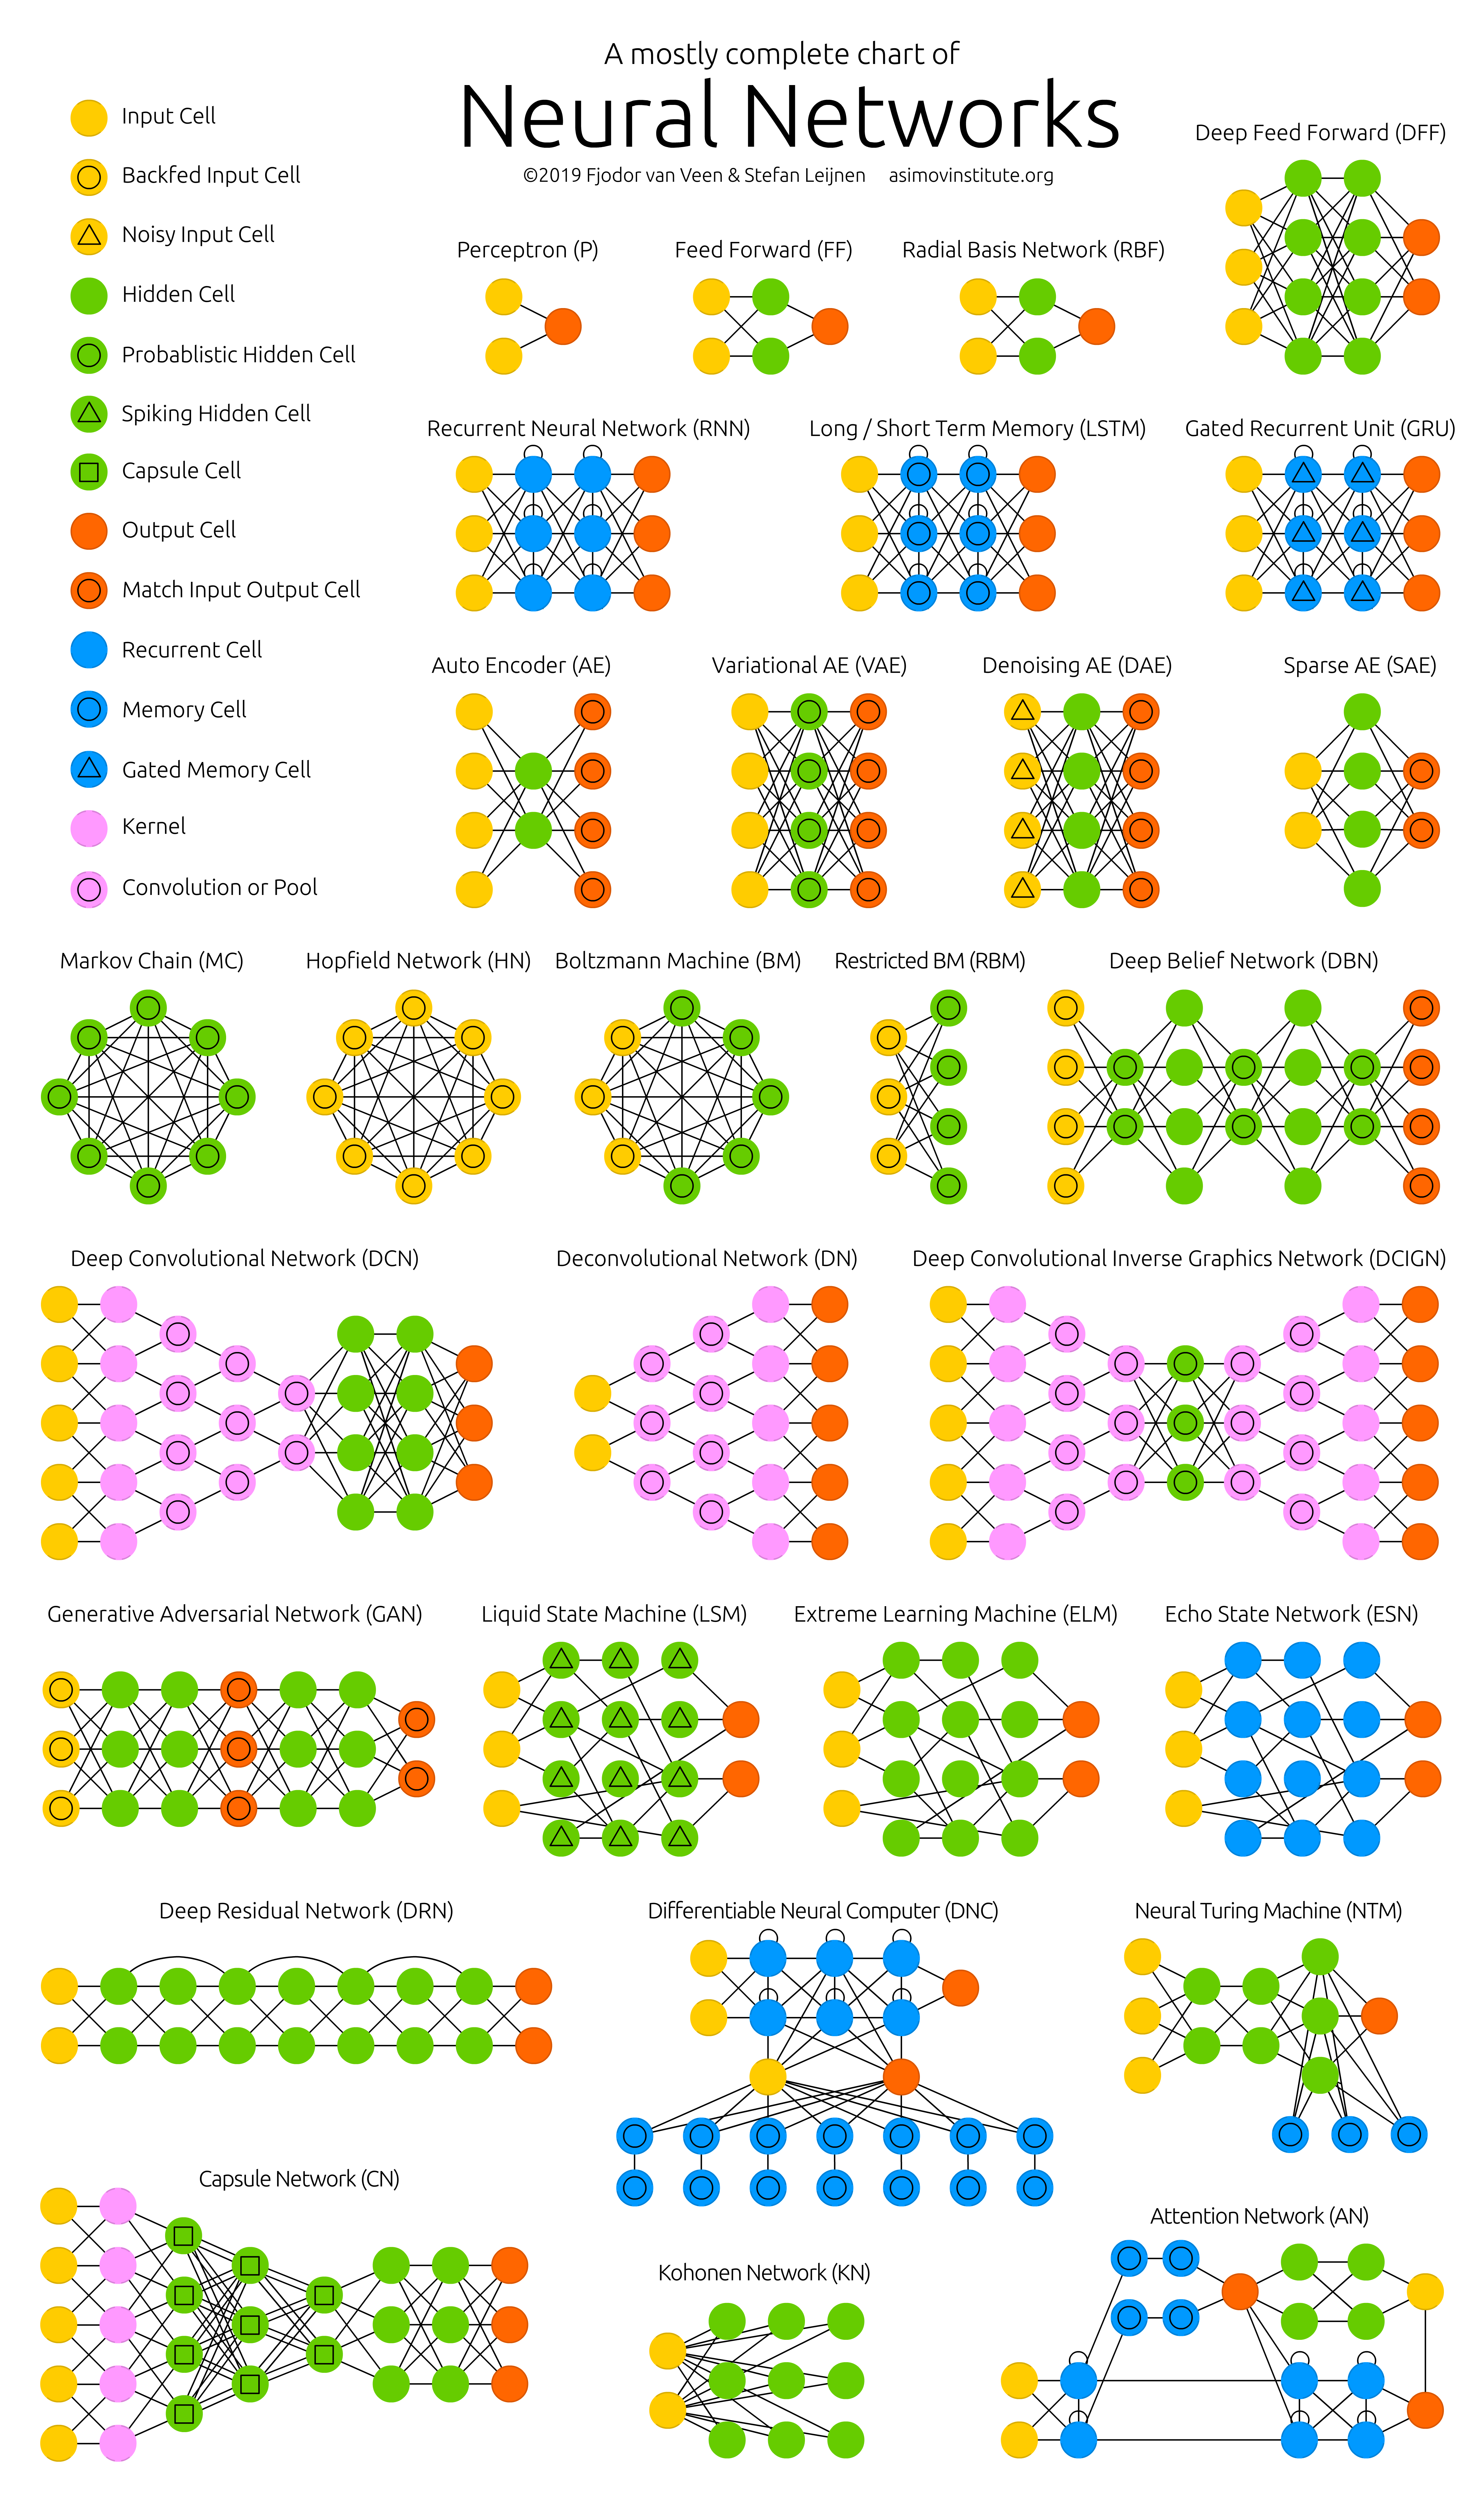
\includegraphics[width=0.65\textwidth]{figures/NeuralNetworkZo19High.png}
    \caption{Topologías de redes neuronales.\\Fuente: \href{https://www.asimovinstitute.org/neural-network-zoo/}{The neural network zoo}}
    \label{fig:NeuralNetworkZo19High}
\end{figure}
% endregion topologías



% region GANs
\subsection{Redes generativas adversariales - \textit{Generative Adversarial Networks (GAN)}}
% TODO: definición
% TODO: usos
% TODO problemas
\begin{figure}[H]
    \centering
    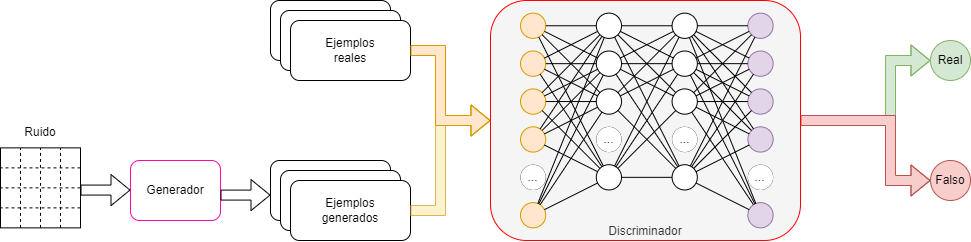
\includegraphics[width=1\textwidth]{figures/chapter02/GANs.drawio.png}
    \caption{Arquitectura de las redes neuronales generativas adversariales.\\Fuente: Elaboración propia.}
    \label{fig:gans-architecture}
\end{figure}
% endregion GANs


% endregion

% region subsection La seguridad de las redes neuronales
\subsection{La seguridad de las redes neuronales}
\label{ch:2:section:state-of-the-art:computer-security-in-neural-networks}

% Dentro de la inteligencia artificial \gls{AI} encontramos el aprendizaje automático \gls{ML} y dentro el aprendizaje profundo \gls{DL}.
% Para el desarrollo de este capítulo limitaremos el alcance del estado del arte de la seguridad informática a los campos relacionados con la inteligencia artificial.

El estado del arte de la seguridad informática es muy complejo, ya que los delincuentes informáticos adoptan nuevas técnicas y tácticas para eludir las medidas de seguridad, esto hace que las ciber amenazas están en constante evolución, también amenaza a las tecnologías que emplean la inteligencia artificial y redes neuronales.

A continuación, se explicarán las distintas amenazas que tiene una red neuronal y como puede ser atacada o implementar defensas, posteriormente analizaremos el estado del arte de la inteligencia artificial que se emplea para mejorar la seguridad informática de los dispositivos y de los usuarios.

\begin{figure}[H]
    \centering
    \centerline{\includesvg[width=1\linewidth]{figures/chapter02/art-architecture.drawio.svg}}
    \caption{Arquitectura de ART.\newline{}Fuente: \href{https://github.com/Trusted-AI/adversarial-robustness-toolbox/wiki/ART-Architecture-and-Roadmap}{GitHub @Trusted-AI/adversarial-robustness-toolbox}}
    \label{fig:art-architecture}
\end{figure}

ART \cite{art2018} consta con 6 módulos específicos para ataque, defensas, estimadores, evaluaciones, métricas y preprocesamiento. Esto podemos verlo en la Figura \ref{fig:art-architecture}
% Eficiencia
% Invisivilidad
% Efectividad

\subsection{Amenazas de \textit{deep learning}}
% region Amenazas de \textit{deep learning}
\begin{figure}[H]
    \centering
    \centerline{\includesvg[width=1\columnwidth]{figures/chapter02/adversarial-threats.drawio.svg}}
    \caption{Amenazas adversariales.\\Fuente: Elaboración propia.}
    \label{fig:art-adversarial-threats}
\end{figure}

Como podemos observar en la Figura \ref{fig:art-adversarial-threats} existen multitud de amenazas, existen cuatro formas de clasificar las amenazas, está clasificación es en función de cómo se altera el comportamiento del modelo.

\subsubsection{Evasión}

Busca explotar las vulnerabilidades de la red neuronal para inducir errores en la capacidad de clasificar o de predecir. Se envía información con perturbaciones mínimas que alteren notablemente la respuesta del modelo.

\begin{enumerate}
    \item \textbf{Caja blanca}: se conoce todo sobre el modelo, arquitectura, pesos, umbrales, formato de entrada de datos y salida, etc. \cite{learning-machine-learning-part-3-attacking}
    \item \textbf{Caja negra}: se desconoce el modelo, arquitectura, pesos, umbrales, pero se conoce el formato de entrada de datos y la respuesta del modelo. \cite{learning-machine-learning-part-3-attacking}
\end{enumerate}

\subsubsection{Envenenamiento}

Los atacantes intentan manipular los datos de entrenamiento con el objetivo de influir en el resultado del aprendizaje del modelo, esto pueden hacerlo desde distintas etapas.

% $$ \sum_{rand}(x)=\left\{clip\left(x+\delta\right)|\delta\in[-5,5]^{H\times W\times3}\right\} $$

\begin{enumerate}
    \item \textit{Label Flipping Attacks} - Ataques de cambio de etiquetas:
    \item \textit{Clean Label Data Poisoning Attack} - Ataques de envenenamiento de datos de etiquetado limpio:
    \item \textit{Backdoor Attack} - Ataques de puerta trasera: los ataques de puerta trasera, ataques que contienen un disparador, estos se pueden clasificar en tres tipos de escenarios.
\end{enumerate}

\paragraph{Label Flipping Attacks}

\paragraph{Clean Label Data Poisoning Attack}

\subparagraph{Feature Collision Attack}

\begin{equation}
    x_{p}={\underset{x}{\mathrm{argmin}}}||f\left(x\right)-f\left(x_{t}\right)||_{2}^{2}+\beta||x-x_{b}||_{2}^{2}
\end{equation}


\subparagraph{Convex Polytope Attack and Bullseye Polytope Attack}

\paragraph{Backdoor Attack}


\subsubsection{Extracción}

Se busca extraer un funcionamiento interno equivalente de la red neuronal, se puede considerar un ataque de ingeniería inversa.

% 
\subsubsection{Inferencia}

\paragraph{Inferencia por Atributos}
\paragraph{Inferencia por Pertenencia}
\paragraph{Inversión de modelos}
\paragraph{Reconstrucción}

% endregion 

\subsection{Defensas contra los ataques en \textit{deep learning}}

\subsubsection{Preprocesamiento}
\subsubsection{Post procesamiento}
\subsubsection{Entrenamiento}
\subsubsection{Transformación}
\paragraph{Evasión}
\paragraph{Envenenamiento}
\subsubsection{Detector}
\paragraph{Evasión}
\paragraph{Envenenamiento}

\subsection{Métricas en los ataques adversariales}

\subsection{Redes neuronales en \textit{Red team} y \textit{Blue team}}

Un buen símil entre la seguridad informática clásica y la seguridad en redes neuronales son los conceptos de equipos de ataque y defensa (``red team'' y ``blue team'').

\begin{figure}[H]
    \centering
    \centerline{\includesvg[width=1\columnwidth]{figures/chapter02/ART-for-red-and-blue-teams.drawio.svg}}
    \caption{Ataques y defensas en redes neuronales.\\Fuente: Elaboración propia.}
    \label{fig:art-for-red-and-blue-teams}
\end{figure}

La idea detrás del aprendizaje automático es la de poder predecir modelos predictivos, para ello se usan conjuntos de datos para el entrenamiento.

Los conjuntos de datos se han de procesar, ya que suelen contener mucho ruido, es decir, información muy poco valiosa, errónea o, por el contrario, una alta dimensionalidad de los datos que puede ser contraproducente por no poder reproducir esas medidas o por la poca información que aportan.

Los ataques al aprendizaje automático o profundo suelen estar dirigidos a las distintas etapas de creación y uso de un modelo.

\begin{itemize}
    \item Alteración de los datos de entrada.
    \item Alteración del proceso de aprendizaje.
    \item Extracción de los datos de entrenamiento.
    \item Bloqueo del modelo.
\end{itemize}

Durante el transcurso del trabajo discutiremos los siguientes ataques y defensas previamente en la sección \nameref{ch:2:section:state-of-the-art:computer-security-in-neural-networks} que se pueden usar en los modelos.

\begin{itemize}
    \item Envenenamiento de datos.
    \item Puerta trasera.
    \item Extracción de datos
    \item Ingeniería inversa.
    \item Evasión.
\end{itemize}

Se puede ser categorizar la seguridad de los modelos con el modelado \gls{STRIDE} de microsoft\footnote{Modelado de amenazas de microsoft \href{https://learn.microsoft.com/es-es/azure/security/develop/threat-modeling-tool-threats}{Enlace}} o con la matriz \gls{MITRE}.

\begin{table}[H]
    \centering
    \small
    \begin{tabularx}{\textwidth}{|l|X|}
        \hline
        \textbf{Amenaza}    & \textbf{Tipo de ataque}                                           \\
        \hline
        Corrupción de datos & Ataques de envenenamiento de datos, ataques de puerta trasera     \\
        Extracción de datos & Ataques de inferencia de membresía, ataques de ingeniería inversa \\
        Denegación          & Ataques de envenenamiento de datos                                \\
        \hline
    \end{tabularx}
    \caption{Amenazas STRIDE relacionadas con la seguridad de la IA}
    \label{tab:amenazas}
\end{table}

% endregion

% region subsection Las redes neuronales para la seguridad informática
\subsection{Las redes neuronales para la seguridad informática}
% TODO: aplicaciones reales de ciberseguridad que usan inteligencia artificial 


% endregion




\subsection{Normativa y estándares}
% https://eur-lex.europa.eu/resource.html?uri=cellar:e0649735-a372-11eb-9585-01aa75ed71a1.0008.02/DOC_1&format=PDF
% https://eur-lex.europa.eu/resource.html?uri=cellar:e0649735-a372-11eb-9585-01aa75ed71a1.0008.02/DOC_2&format=PDF

% Según la unión europea toda la seguridad es este apartado :ok: 
% (51) La ciberseguridad es fundamental para garantizar que los sistemas de IA resistan a las actuaciones de terceros maliciosos que, aprovechando las vulnerabilidades del sistema, traten de alterar su uso, conducta o funcionamiento o de poner en peligro sus propiedades de seguridad. Los ciberataques contra sistemas de IA pueden dirigirse contra elementos específicos de la IA, como los conjuntos de datos de entrenamiento (p. ej., contaminación de datos) o los modelos entrenados (p. ej., ataques adversarios), o aprovechar las vulnerabilidades de los elementos digitales del sistema de IA o la infraestructura de TIC subyacente. Por lo tanto, para asegurar un nivel de ciberseguridad adecuado a los riesgos, los proveedores de sistemas de IA de alto riesgo deben adoptar medidas adecuadas teniendo también en cuenta, cuando proceda, la infraestructura de TIC subyacente.









% https://www.youtube.com/@felipebravom



% Feb 1990: Generative Adversarial Networks / Curiosity Generative Adversarial Networks (GANs) have become very popular.[MOST] They were first published in 1990 in Munich under the moniker Artificial Curiosity. [AC90-20][GAN1] Two dueling NNs (a probabilistic generator and a predictor) are trying to maximize each other's loss in a minimax game.[AC](Sec. 1) The generator (called the controller) generates probabilistic outputs (using stochastic units[AC90] like in the much later StyleGANs[GAN2]). The predictor (called the world model) sees the outputs of the controller and predicts environmental reactions to them. Using gradient descent, the predictor NN minimizes its error, while the generator NN tries to make outputs that maximize this error: one net's loss is the other net's gain.[AC90] (The world model can also be used for continual online action planning.[AC90][PLAN2-3][PLAN])
% 4 years before a 2014 paper on GANs,[GAN1] my well-known 2010 survey[AC10] summarised the generative adversarial NNs of 1990 as follows: a "neural network as a predictive world modelis used to maximize the controller's intrinsic reward, which is proportional to the model's prediction errors" (which are minimized).
% The 2014 GANs are an instance of this where the trials are very short (like in bandit problems) and the environment simply returns 1 or 0 depending on whether the controller's (or generator's) output is in a given set.[AC20][AC][T22](Sec. XVII)
% Other early adversarial machine learning settings[S59][H90] were very different—they neither involved unsupervised NNs nor were about modeling data nor used gradient descent.
% The 1990 principle has been widely used for exploration in Reinforcement Learning[SIN5][OUD13] [PAT17][BUR18] and for synthesis of realistic images,[GAN1,2] although the latter domain was recently taken over by Rombach et al.'s Latent Diffusion, another method published in Munich,[DIF1] building on Jarzynski's earlier work in physics from the previous millennium[DIF2]  and more recent papers.[DIF3-5]
% In 1991, I published yet another ML method based on two adversarial NNs called Predictability Minimization for creating disentangled representations of partially redundant data, applied to images in 1996.
